\chapter{Número Envoltório $P_3$ em Grafos de diâmetro 2}
\label{envoltoria}

Explorando as propriedades dos grafos de diâmetro 2 na convexidade $P_3$, podemos obter resultados interessantes para os parâmetros de número envoltório e número de Carathéodory. Veremos nessa seção os limites identificados neste trabalho para o número envoltório.

Analisaremos alguns grafos de diâmetro 2 em função do grau máximo e da quantidade de vértices. Seja $G$ um grafo estrela contendo $n-1$ vértices de grau 1.  Observe que para todo $v\in V(G)$ com $d(v)=1$, ou $v \in S$ ou $v \notin H(S)$. Logo, todo $v \in V(G)$ com grau 1 pertence a um conjunto envoltório. Portanto, em um grafo estrela com $n$ vértices o conjunto envoltório mínimo precisa conter todos os vértices de grau 1, consequentemente o número envoltório da estrela é $n-1$. Portanto, podemos estabelecer um primeiro limite do número envoltório para grafos de diâmetro 2.

\begin{observation}
Se $G$ é um grafo de diâmetro 2 com vértice de corte, então $h(G) \le n-1$.
\label{theor-d2-n-1}
\end{observation}

Esse limite é bom, porém não é justo. Na Figura~\ref{fig-exemplos-n-1} temos 3 grafos de 9 vértices com $\Delta=n-1$. No grafo (a) temos um grafo estrela com $h(G)=n-1=8$ e atingindo o limite da Observação \ref{theor-d2-n-1}. Já o grafo em (b) possui $h(G)=4<n-1$. 

Note que o grafo (b) da Figura~\ref{fig-exemplos-n-1} tem um vértice de corte $c$ $\omega(G-c)=4$. Então se $G$ possui um vértice de corte podemos melhorar o limite apresentado na Observação~\ref{theor-d2-n-1}.

\begin{proposition}
%Se $G$ é um grafo de diâmetro 2 com vértice de corte $c$ então $h(G) \leq \omega(G-c)$. 
Se $G$ é um grafo de diâmetro 2 com vértice de corte $c$ então $h(G) = \omega(G-c)$. 
\end{proposition}
\begin{proof}
Seja $G$ um grafo de diâmetro 2 com vértice de corte $v$, e considere $G^\prime=G-e$. Como $v$ é vértice de corte temos que $G^\prime$ é desconexo com $k=\omega(G^\prime)\geq 2$ componentes. Façamos $S$ um subconjunto de $V(G^\prime)$ contendo exatamente um vértice de cada componente conexa de $G'$. Observe que $|S|=k$. Iremos mostrar que para todo $u \in V(G)\backslash S$, $u \in H(S)$. Consideraremos dois casos:

{\it Caso 1: $u=v$.}\\
Como $u$ é vértice de corte, $G^\prime$ possui ao menos duas componentes conexas. Então $u \in H(\{u_1, u_2\})$  tal que $u_1v, u_2v \in E(G')$ e $u_1$ e $u_2$ pertençam a componentes conexas distintas de $G$.

{\it Caso 2: $u \in C_i$, onde $C_i$ é uma componente de $G'$.}\\ 
Considere o caminho $P=u,u_1, u_2,\cdots, u_\ell$, $\ell \geq 1$, pertencente a componente $C_i$ tal que $u_\ell \in S$. Pelo caso anterior temos que $v \in H(S)$ e $v \in I(S)$. Como $v$ é vértice de corte de $G$ e $G$ é um grafo de diâmetro 2, pela Proposição \ref{pro-diam-2-itemd} $v$ é adjacente a todos os vértice de $G$, incluindo todos os vértices do caminho $P$. Assim, $u_{\ell-1} \in I^2(S)$, $u_{\ell-2} \in I^3(S)$ e assim sucessivamente, $u \in I^{|P|-2}$. Logo $u \in H(S)$.

Com isso temos que $S$ é um conjunto envoltório de $G$ de cardinalidade $\omega(G-c)$, portanto $h(G) \leq \omega(G-c)$.

Agora demonstraremos que $h(G)\ge G-c$, seja $S$ um conjunto envoltório de $G$, $S$ deve possuir no mínimo um vértice pertencente a cada componente de conexa de $G-c$. Supomos por contradição que $S$ é um conjunto envoltório de $G$ e existe uma componente conexa $G_t$ de $G-c$, tal que $V(G_t) \subseteq H(S)$ e $\not \exists v \in S|v\in V(G_t)$.

Por definição ao menos um dos vértices de $G_t$ possuem 2 vizinhos em $H(S)$ externos a $G_t$, como $c\in H(S)$, podemos afirmar que existe um outro vértice $v_x \in H(S)$ tal que $v_x \ne c$. Como $v_x \not \in V(G_t)$, ele só pode estar em outra componente conexa $G_x$ diferente de $G_t$, e $v_x$ tem um caminho induzido por $H(S)$ a um vértice $s_0|s_0\in S$, com isso temos outro caminho induzido de $v_t,v_x,\dots,s_0$ tal que esse caminho não passa por $c$, então $G_x$ e $G_t$ são conexos em $G-c$, o que é uma contradição, com isso temos que $h(G)\ge \omega(G-c)$.

Com isso temos a demonstração do limite superior e inferior do número envoltório em grafos de diâmetro 2 com vértice de corte, provamos assim a igualdade $h(G) = \omega(G-c)$.
\end{proof}

%ao passo que o grafo (b) não possui vértices pendurados mas possui um vértice de corte e seu número de envoltória é 4, e o último grafo que é uma roda que não possui vértice de corte ou pendurados, cujo número envoltório é 2. Quando o grafo possui um vértice $v$ tal que $d(v)=n-1$ esse grafo pode conter um vértice de corte ou vértices pendurados, tendo assim um limite muito amplo.

%Agora, seja $G$ um grafo de diâmetro 2 que contenha vértice de corte. Então pela Proposição \ref{pro-diam-2-itemd} $\Delta(G)=n-1$.
%um grafo com com  para estabelecer um limite para o número de envoltória, pois podemos ter vértice de corte e vértices de grau 1. Em um grafo estrela o número de envoltória é a quantidade de folhas, em um grafo roda o número de envoltória é 2, e ao passo que alguns de seus subgrafos tem envoltória maior que 2 e menor do que $n-1$, tais como os grafos do exemplo na Figura~\ref{fig-exemplos-n-1}.

\begin{figure}[h]
\centering
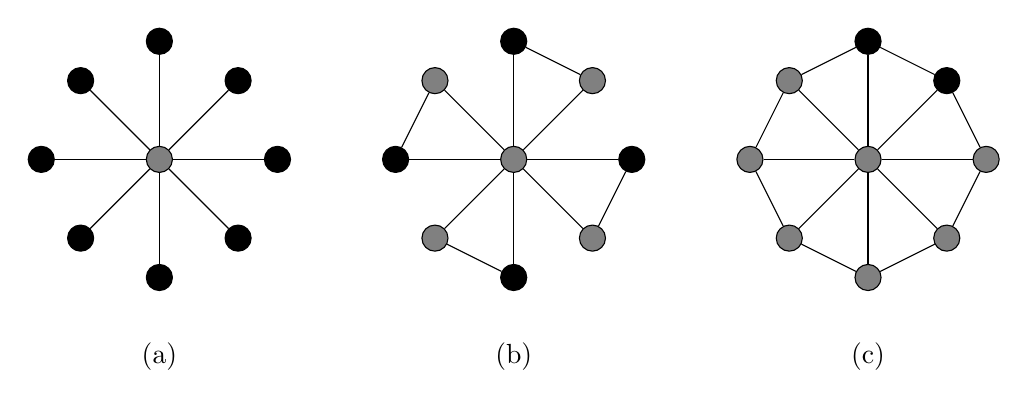
\begin{tikzpicture}
\node[circle,draw,fill=black!50] (v1) at (-13.5,-1) {};
\node[circle,draw,fill] (v3) at (-13.5,0.5) {};
\node[circle,draw,fill] (v9) at (-15,-1) {};
\node[circle,draw,fill] (v7) at (-13.5,-2.5) {};
\node[circle,draw,fill] (v5) at (-12,-1) {};
\node[circle,draw,fill] (v8) at (-14.5,-2) {};
\node[circle,draw,fill] (v6) at (-12.5,-2) {};
\node[circle,draw,fill] (v4) at (-12.5,0) {};
\node[circle,draw,fill] (v2) at (-14.5,0) {};
\draw  (v1) edge (v2);
\draw  (v1) edge (v3);
\draw  (v1) edge (v4);
\draw  (v1) edge (v5);
\draw  (v1) edge (v6);
\draw  (v7) edge (v1);
\draw  (v1) edge (v8);
\draw  (v1) edge (v9);

\node[circle,draw,fill=black!50] (v31) at (-9,-1) {};
\node[circle,draw,fill] (v33) at (-9,0.5) {};
\node[circle,draw,fill] (v39) at (-10.5,-1) {};
\node[circle,draw,fill] (v37) at (-9,-2.5) {};
\node[circle,draw,fill] (v35) at (-7.5,-1) {};
\node[circle,draw,fill=black!50] (v38) at (-10,-2) {};
\node[circle,draw,fill=black!50] (v36) at (-8,-2) {};
\node[circle,draw,fill=black!50] (v34) at (-8,0) {};
\node[circle,draw,fill=black!50] (v32) at (-10,0) {};
\draw  (v31) edge (v32);
\draw  (v31) edge (v33);
\draw  (v31) edge (v34);
\draw  (v31) edge (v35);
\draw  (v31) edge (v36);
\draw  (v37) edge (v31);
\draw  (v31) edge (v38);
\draw  (v31) edge (v39);

\node[circle,draw,fill=black!50] (v21) at (-4.5,-1) {};
\node[circle,draw,fill] (v23) at (-4.5,0.5) {};
\node[circle,draw,fill=black!50] (v29) at (-6,-1) {};
\node[circle,draw,fill=black!50] (v27) at (-4.5,-2.5) {};
\node[circle,draw,fill=black!50] (v25) at (-3,-1) {};
\node[circle,draw,fill=black!50] (v28) at (-5.5,-2) {};
\node[circle,draw,fill=black!50] (v26) at (-3.5,-2) {};
\node[circle,draw,fill] (v24) at (-3.5,0) {};
\node[circle,draw,fill=black!50] (v22) at (-5.5,0) {};
\draw  (v21) edge (v22);
\draw  (v21) edge (v23);
\draw  (v21) edge (v24);
\draw  (v21) edge (v25);
\draw  (v21) edge (v26);
\draw  (v27) edge (v21);
\draw  (v21) edge (v28);
\draw  (v21) edge (v29);
\draw  (v23) edge (v24);
\draw  (v24) edge (v25);
\draw  (v26) edge (v25);
\draw  (v27) edge (v26);
\draw  (v28) edge (v29);
\draw  (v28) edge (v27);
\draw  (v22) edge (v29);
\draw  (v23) edge (v22);

\draw  (v34) edge (v33);
\draw  (v36) edge (v35);
\draw  (v37) edge (v38);
\draw  (v39) edge (v32);
\node at (-13.5,-3.5) {(a)};
\node at (-9,-3.5) {(b)};
\node at (-4.5,-3.5) {(c)};
 \end{tikzpicture}
\caption{Exemplos de grafos de diâmetro 2 e $\Delta=n-1$}
\label{fig-exemplos-n-1}
\end{figure}



Se $G$ é um grafo de diâmetro 2 e $\Delta <n-1$ logo temos 2 restrições: 
%essas propriedades estão nos fundamentos (propriedades de grafos de diâmetro 2
não temos vértice de corte ou vértices de grau um. Com essas restrições
melhorias no limite do número envoltório podem ser estabelecidas.


\begin{lemma}
     \label{hs-dominante-envoltorio}
     Seja $G$ um grafo de diâmetro 2 biconexo e $S^\prime \subseteq V(G)$. 
     Se $H(S^\prime)$ é um conjunto dominante, então $G$ possui um conjunto envoltório $S$ tal que  $S=S^\prime \cup \{v\}$ para todo $v\in V(G) \setminus H(S^\prime)$.
\end{lemma}
\begin{proof}
Seja $G$ um grafo de diâmetro 2 biconexo tal que $H(S')$ é um conjunto dominante. Observe que todo $v \in V(G)\setminus H(S^\prime)$ possui um único vizinho em $H(S')$. Considere $S=S' \cup \{v\}$, tal que $v \in  V(G) \setminus H(S^\prime)$. Vamos provar que $S$ é um conjunto envoltório mostrando que todo vértice $u \in V(G)\setminus H(S^\prime)$ pertencerá ao fecho convexo de $S$. Dividimos a prova em dois casos.

{\it Caso 1: $uv \in E(G)$}. Como $v \in S$ e existe um $w \in H(S')$, tal que $uw \in E(G)$, temos que $u \in H(S)$.\\

{\it Caso 2: $uv \notin E(G)$}. Como $G$ tem diâmetro 2 existe um vértice $w$ tal que $uw, wv \in E(G)$. Considere que $w \in V(G)\setminus H(S')$. Pelo Caso 1 $w \in H(S)$ pois $vw \in E(G)$. Como $u$ possui um único vizinho em $H(S')$ e $uw \in E(G)$, temos que $u \in H(S)$. Por fim, Considere $w \in H(S')$. Sabemos que $w$ é o único vértice em $H(S')$ tal que $uw, wv \in E(G)$. Como $G$ é conexo e não tem vértice de corte, existe um caminho $P= v, v_1, v_2, \cdots,v_n, u$ em $G$ que não passa por $w$. Então como $v v_1 \in E(G)$ e existe $v^{\prime}_{1} \in H(S')$, tal que $v^{\prime}_{1}v_1 \in E(G)$, temos que $v_1 \in I[S]$. Analogamente como $v_1v_2 \in E(G)$ e existe $v^{\prime}_{2} \in H(S')$ tal que $v^{\prime}_{2}v_2 \in E(G)$, temos que $v_2 \in I^{2}[S]$. Assim, sucessivamente como $v_n u \in E(G)$ e existe $v^{\prime}_{n} \in H(S')$, tal que $v^{\prime}_{n}v_n \in E(G)$, obtemos $u \in I^{n+1}[S]$.\\

Veja ilustração dos casos na Figura \ref{fig-caso-final-hs-dominate}. Como em todos os casos o vértice $u$ pertencerá ao fecho de $S$, com $S= S' \cup \{v\}$, $H(S')$ um conjunto dominante e $v \notin H(S')$, temos que $S$ é um conjunto envoltório.



%Supomos por contradição que $S$ não é um conjunto envoltório e então existe um vértice $u$ tal que $u\not\in H(S)$. Se $u$ e $v$ são adjacentes, como $H(S^\prime)$ é um conjunto dominante temos que $u\in H(S)$, que é uma contradição. Se $u$ e $v$ não são adjacentes e pela Proposição \ref{pro-diam-2-itema} existe um vértice $w\in V(G)$, tal que $w$ é adjacente a $u$ e $v$. Se $w\in V(G)\setminus H(S^\prime)$, então $w \in H(S)$ e consequentemente $u \in H(S)$, uma contradição. Assim, $w \in H(S')$ é um vizinho em comum a $u$ e $v$ e $\not\exists z\in V(G)\setminus H(S^\prime)$ tal que $uz, vz \in E(G)$. Logo, $u$ e $v$ não possuem vizinhos em comum em $V(G)\backslash H(S')$. Desde que $G$ tem grau mínimo pelo menos 2, $u$ e $v$ possuem pelo menos mais um vizinho cada, necessariamente em $V(G) \setminus H (S^\prime)$, denotados por $u^\prime\in N(u)$ and $ v^\prime\in N(v)$.

%{\it Caso 1: $u^\prime, v^\prime\in V(G)\setminus H(S^\prime)$ são adjacente}\\
%Então existe um caminho $vv^\prime u^\prime u$. Como $H(S^\prime)$ é um conjunto dominante então $v^\prime \in H(S)$, $u^\prime \in H(S)$ e consequentemente $u \in H(S)$, uma contradição.

%{\it Caso 2: $u^\prime$,$v^\prime$ não são adjacentes} \\
%Então existe $w^\prime \in V(G) \setminus H(S^\prime)$, tal que a distância $d(v,u^\prime)>2$ e $d(u,v^\prime)>2$, uma contradição pois $G$ tem diâmetro 2.

%{\it Caso 3: $u^\prime$,$v^\prime$ não são adjacentes e não existem os caminhos $u-v$, $u^\prime-v$ and $u-v^\prime$ in $V(G)\setminus H(S^\prime)$.}\\

%Sabemos que existe $w^\prime \in H(S^\prime)$ tal que $w=w^\prime$ then $w\in H(S^\prime)$ and $\{u,v,u^\prime,v^\prime\}$ has no more adjacent vertices in $H(S^\prime)$ and $V(G)\setminus H(S^\prime)$. Thus, $w$ is a cut vertex and $H(S^\prime)$, $\{u,u^\prime\}$ and $\{v,v^\prime \}$ are disconnected components of $G-w$, if G has cut vertex then $\Delta = n-1$, which is a contradiction.

%So the result follows.



%então temos um vértice $u\not\in H(S^\prime\{v\})$ e $u,v\not\in H(S^\prime)$, se $u$ e $v$ são vizinhos então $u \in H(S^\prime\cup\{v\})$, o que é uma contradição. Caso $u$ e $v$ não são adjacentes então existe $w\in V(G)$ tal que $w$ é adjacente a $u$ e $v$ analisaremos individualmente as possibilidades de $w$:

%    Caso 1: Se $\exists w \in V(G) \setminus H(S^\prime)$ então necessariamente $u \in H(S^\prime\cup\{v\})$, contradizendo a suposição.    
%    Caso 2: Se $\not \exists w \in V(G) \setminus H(S^\prime)$ então $w \in H(S^\prime)$ e $u,v$ não tem adjacência com outros vértices de $H(S^\prime)$. 
%    Como G não possui vértices isolados $u$ e $v$ tem ao menos mais um vizinho cada, necessariamente em $V(G)\setminus H(S^\prime)$, tal que $u^\prime \in N(u)$ e $v^\prime \in N(v)$.    

%    Caso 2.1: Existe $u^\prime,v^\prime\in V(G)\setminus H(S^\prime)$ adjacentes , então existe um caminho $v v^\prime u^\prime u$, em que todos os vértices estão em $V(G)\setminus H(S^\prime)$ e tem um vértice adjacente em $H(S^\prime)$, dessa forma $u \in H(S^\prime \cup \{v\})$ o que é contradição a suposição.    

%    Caso 2.2: Não existe $u^\prime$ e $v^\prime$ adjacentes então existe $w^\prime \in H(S^\prime)$, porém a distância $d(v,u^\prime)>2$ e $d(u,v^\prime)>2$ o que é uma contradição.    

%   Caso 2.3: Não existe $u^\prime$ e $v^\prime$ adjacentes então existe $w^\prime \in H(S^\prime)$ tal que $w=w^\prime$ então $w \in H(S^\prime)$ e $u,v,u^\prime,v^\prime$ não tem adjacência com outros vértices de $H(S^\prime)$, dessa forma $w$ é um vértice de corte e $H(S^\prime)$, $\{u,u^\prime\}$ e $\{v,v^\prime\}$ são componentes desconexas, o que é uma contradição pois se G possui vértice de corte então $\Delta(G)=n-1$.
%    Por contradição temos que a proposição ~\ref{hs-dominante-envoltorio} é válida.

%    Caso 1: Se $\exists w \in V(G) \setminus H(S^\prime)$ então necessariamente $u \in H(S^\prime\cup\{v\})$, contradizendo a suposição.
    
    %Caso 2: Se $\not \exists w \in V(G) \setminus H(S^\prime)$ então $w \in H(S^\prime)$ e $u,v$ não tem adjacência com outros vértices de $H(S^\prime)$. 
    %Como G não possui vértices isolados $u$ e $v$ tem ao menos mais um vizinho cada, necessariamente em $V(G)\setminus H(S^\prime)$, tal que $u^\prime \in N(u)$ e $v^\prime \in N(v)$.
    
    %Caso 2.1: Existe $u^\prime,v^\prime\in V(G)\setminus H(S^\prime)$ adjacentes , então existe um caminho $v v^\prime u^\prime u$, em que todos os vértices estão em $V(G)\setminus H(S^\prime)$ e tem um vértice adjacente em $H(S^\prime)$, dessa forma $u \in H(S^\prime \cup \{v\})$ o que é contradição a suposição.
    
    %Caso 2.2: Não existe $u^\prime$ e $v^\prime$ adjacentes então existe $w^\prime \in H(S^\prime)$, porém a distância $d(v,u^prime)>2$ e $d(u,v^prime)>2$ o que é uma contradição. 
   
   %Caso 2.3: Não existe $u^\prime$ e $v^\prime$ adjacentes então existe $w^\prime \in H(S^\prime)$ tal que $w=w^\prime$ então $w \in H(S^\prime)$ e $u,v,u^\prime,v^\prime$ não tem adjacência com outros vértices de $H(S^\prime)$, dessa forma $w$ é um vértice de corte e $H(S^\prime)$, $\{u,u^\prime\}$ e $\{v,v^\prime\}$ são componentes desconexas, o que é uma contradição pois $G$ não possui vértice de corte.
    %Por contradição, temos que o Lema ~\ref{hs-dominante-envoltorio} é válido.
\end{proof}

\begin{figure}[h]
\centering
\begin{tikzpicture}
\node (v1) at (-12.0729,6.5067) {};
\node (v5) at (-12.0729,5.5067) {};  
\node[draw,circle,inner sep=0pt,minimum size=5pt,label=right:$v$] (v) at (-10.3012,6.8026) {};
\node[draw,circle,inner sep=0pt,minimum size=5pt,label=right:$u$] (u) at (-10.2191,5.2937) {};
\node[draw,ellipse,minimum width=1.5cm,minimum height=2.5cm,label={\scriptsize $H(S^\prime)$}] (v6) at (-11.9,6) {};
\node[draw,ellipse,minimum width=1.5cm,minimum height=2.5cm,label={\scriptsize $V(G) \setminus H(S^\prime)$}] at (-10.1,6) {};
\draw  (v1) edge (v);
\draw  (v5) edge (u);
\draw  (v) edge (u);


\node[draw,circle,inner sep=0pt,minimum size=5pt,label=right:$v$] (vc) at (-12.4,2.8) {};
\node[draw,circle,inner sep=0pt,minimum size=5pt,label=right:$u$] (uc) at (-12.4,1) {};
\node[draw,ellipse,minimum width=1.5cm,minimum height=2.5cm,label={\scriptsize $H(S^\prime)$}] at (-14,2) {};
\node[draw,ellipse,minimum width=1.5cm,minimum height=2.5cm,label={\scriptsize $V(G) \setminus H(S^\prime)$}] at (-12.2,2) {};
\node[draw,circle,inner sep=0pt,minimum size=5pt,label=right:$w^\prime$] (v4) at (-12.5,2) {};
\draw  (uc) edge (v4);
\draw  (v4) edge (vc);


\node (v9) at (-14,2.5) {};
\node (v10) at (-14,1.5) {};
\node[draw,circle,inner sep=0pt,minimum size=5pt,label=right:$v$] (vc2) at (-8.5,3) {};
\node[draw,circle,inner sep=0pt,minimum size=5pt,label=right:$u$] (uc2) at (-8.5,1) {};
\node[draw,circle,inner sep=0pt,minimum size=5pt,label=right:$w$] (wc2) at (-10,2) {};
\node[draw,ellipse,minimum width=1.5cm,minimum height=2.5cm,label={\scriptsize $H(S^\prime)$}] at (-10.1,2) {};
\node[draw,ellipse,minimum width=1.5cm,minimum height=2.5cm,label={\scriptsize $V(G) \setminus H(S^\prime)$}] at (-8.4,2) {};
\node at (-10.2,2.7) {};
\node at (-10.1,1.5) {};
\draw  (vc2) edge (wc2);
\draw  (uc2) edge (wc2);

\node at (-11,4.5) {Caso 1};
\node at (-13.1,0.5) {Caso 2a};
\node at (-9.2,0.5) {Caso 2b};

\draw  (v9) edge (vc);
\draw  (uc) edge (v10);
\draw[snake=zigzag,dashed]  (vc2) edge (uc2);
\node at (-8,2) {$P_{vu}$};
\end{tikzpicture}
\caption{Casos da prova do Lema~\ref{hs-dominante-envoltorio}}
\label{fig-caso-final-hs-dominate}
\end{figure}

%  \begin{coro}\label{coro-corte} 
% Se $G$ é um grafo de diâmetro 2 biconexo e $C_t \subseteq V(G)$ é um corte mínimo de vértices, 
% então $h(G) \le |C_t|+ 1$.
% \end{coro}
% \begin{proof}

% \end{proof}

\begin{coro}\label{coro-deltinha} Se $G$ é um grafo de diâmetro 2 biconexo então $h(G) \le \delta + 1$.
\end{coro}
\begin{proof}
Pela Proposição \ref{pro-diam-2-itemb} para todo $v \in V(G)$, $N(v)$ é um conjunto dominante. Seja $v \in V(G)$ tal que $d(v)= \delta$. Pelo Lema \ref{hs-dominante-envoltorio} temos que $S=N(v) \cup \{u\}$, com $u \in V(G) \setminus N[v]$, é um conjunto envoltório. Portanto, $h(G) \leq \delta+1$.  

Como $\exists v \in V(G)$ tal que $d(v)=\delta$, assim temos que $N(v)$ é um cojunto dominante. Fazendo $S^\prime=N(v)$ então pelo Lema ~\ref{hs-dominante-envoltorio} temos que $G$ possui um conjunto envoltório $S=S^\prime \cup \{u\}$ com cardinalidade $|S|=|S^\prime|+1=\delta+1$, com isso temos um limite superior para o número envoltório de grafos de diâmetro 2 biconexo. 
\end{proof}

Como exemplo, temos os grafos $G_7$ e $C_5$ na Figura~\ref{fig:exemplos-d-deltinha}, que são grafos de diâmetro 2 e biconexo. Observe que $\delta=2$ e que $d(v_{\delta})=2$ nos dois grafos. Pelo Corolário ~\ref{coro-deltinha}, temos que o limite superior para $h(G)$ é $\delta+1=3$ e que $S=\{N(v_{\delta}), u\}$ é um conjunto envoltório. Note que nos grafos ilustrados não existem conjuntos envoltórios com cardinalidade menor. Logo, os grafos exemplificados atingem a igualdade do limite apresentado. Esse limite mostra-se melhor do que o estabelecido na Observação~\ref{theor-d2-n-1}.

%Theorem4. If G is a diameter-2 graph of order n, then γt(G) ≤ 1+√n ln(n).
%Desormeaux, W. J., Haynes, T. W., Henning, M. A., & Yeo, A. (2013). Total Domination in Graphs with Diameter 2, 91–103. https://doi.org/10.1002/jgt
Desormeaux et. al. \cite{Desormeaux2013} provaram resultados relacionados à dominação total em grafos de diâmetro 2, Henning et. al \cite{Henning2009} traz resultados para grafos planares de diâmetro 2.  Denote por $\gamma_t(G)$ a cardinalidade do menor conjunto dominante total.

\begin{theorem}\cite{Henning2009} 
\label{teo-desormeaux0}
Se $G$ um grafo de diâmetro 2 e planar então $\gamma_t(G) \leq 3$. 
\end{theorem}

\begin{coro} 
Se $G$ é um grafo de diâmetro 2 biconexo e planar, então $h(G) \le  4$.
\label{coro-domina0}
\end{coro}
\begin{proof}
Sabemos que, pelo Lema \ref{hs-dominante-envoltorio}, $h(G) \leq S' + 1$, tal que $S'$ é um conjunto dominante. Logo, se $G$ possui um conjunto dominante total de tamanho no máximo $3$, concluímos que $h(G) \leq 4$.
\end{proof}

\begin{theorem}\cite{Desormeaux2013} 
\label{teo-desormeaux1}
Se $G$ um grafo de diâmetro 2 de ordem $n$ então $\gamma_t(G) \leq 1 + \sqrt{n \ln(n)}$. 
\end{theorem}

O Teorema \ref{teo-desormeaux1} pode ser utilizado para melhorar o limite estabelecido no Corolário \ref{coro-deltinha}.

\begin{coro} 
Se $G$ é um grafo de diâmetro 2  biconexo, então $h(G) \le  \sqrt{n\ln(n)} + 2$.
\label{coro-domina1}
\end{coro}
\begin{proof}
Sabemos que, pelo Lema \ref{hs-dominante-envoltorio}, $h(G) \leq S' + 1$, tal que $S'$ é um conjunto dominante. Logo, se $G$ possui um conjunto dominante total de tamanho no máximo $1+ \sqrt{n \ln(n)}$, concluímos que $h(G) \leq 2+ \sqrt{n \ln(n)}$.
\end{proof}

Ainda em Desormeaux et. al. \cite{Desormeaux2013} provaram resultados para o número de dominação total dependendo de valores para o grau mínimo de $G$.

\begin{theorem}\cite{Desormeaux2013} 
\label{teo-desormeaux2}
Seja $G$ um grafo de diâmetro 2 de ordem $n$. Se $\delta \geq \sqrt{n} \ln(n)$, então $\gamma_t(G) \leq 1 + \sqrt{n}$.
\end{theorem}

Com o resultado do Teorema \ref{teo-desormeaux2} podemos melhorar um ainda mais o limite para o número envoltório de grafos de diâmetro 2 biconexo.

\begin{coro}
\label{coro-domina2}
Seja $G$ um grafo de diâmetro 2 biconexo. Se $\delta \ge \sqrt[]{n}ln(n)$ então $h(G) \le \sqrt[]{n} + 2$.
\end{coro}
\begin{proof} 
Segundo o Teorema \ref{teo-desormeaux2} se $\delta(G) \geq \sqrt{n} \ln(n)$ então existe um conjunto dominante total, $S'$, tal que $|S'|\leq \sqrt[]{n} + 1$. Novamente, pelo Lema \ref{hs-dominante-envoltorio} $h(G) \leq \sqrt[]{n} + 2$.
\end{proof}



%Necessidade de exemplos para: b e c?


\begin{figure}[h]
\centering
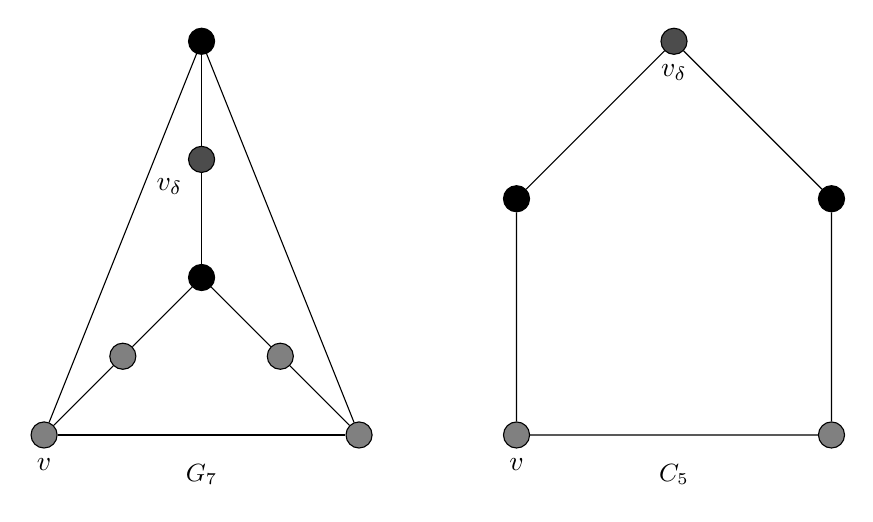
\begin{tikzpicture}
  \node[circle,draw,fill=black!70,label=below left:$v_\delta$] (v1) at (-6,3.5) {};
  \node[circle,draw,fill] (v3) at (-6,2) {};
  \node[circle,draw,fill=black!50] (v4) at (-7,1) {};
  \node[circle,draw,fill=black!50] (v5) at (-5,1) {};
  \node[circle,draw,fill=black!50] (v6) at (-4,0) {};
  \node[circle,draw,fill=black!50,label=below:$v$] (v7) at (-8,0) {};
  \node[circle,draw,fill] (v8) at (-6,5) {};

  \draw  (v8) edge (v1);
  \draw  (v1) edge (v3);
  \draw  (v3) edge (v4);
  \draw  (v3) edge (v5);
  \draw  (v5) edge (v6);
  \draw  (v7) edge (v4);
  \draw  (v7) edge (v8);
  \draw  (v8) edge (v6);
  \draw  (v7) edge (v6);
  
  \node[circle,draw,fill=black!70,label=below:$v_\delta$] (v9) at (0,5) {};
  \node[circle,draw,fill] (v10) at (2,3) {};
  \node[circle,draw,fill=black!50] (v11) at (2,0) {};
  \node[circle,draw,fill=black!50,label=below:$v$] (v12) at (-2,0) {};
  \node[circle,draw,fill] (v13) at (-2,3) {};
  
  \draw (v9) -- (v10) -- (v11) -- (v12) -- (v13) -- (v9);
  
  \node at (-6,-0.5) {\small $G_7$};
  \node at (0,-0.5) {\small $C_5$};
   \end{tikzpicture}
\caption{Exemplos de grafos com $h(G)=\delta(G)+1$ }
\label{fig:exemplos-d-deltinha}
\end{figure}

Observe que os limites dados pelos Corolários \ref{coro-deltinha}, \ref{coro-domina1} e \ref{coro-domina2} não se mostram interessantes quando $\delta$ alcança seu valor máximo, por exemplo, quando temos um grafo regular e $\delta=\Delta$. Para exemplificar, considere o grafo $G$, Hoffman-Singleton~\cite{Hoffman1960}, que é um grafo de diâmetro 2, 7-regular, com 50 vértices. Pelo Corolário \ref{coro-deltinha}, $h(G)\leq 8$. Aplicando o Corolário \ref{coro-domina1} $h(G) \leq 15$ e pelo Corolário \ref{coro-domina2} $h(G) \leq 9$. Entretanto, computacionalmente, verificamos o menor conjunto envoltório do grafo de Hoffman-Singleton tem cardinalidade 4.  

Para aperfeiçoar esse limite vamos apresentar um algoritmo de tempo polinomial que fornece um conjunto dominante com cardinalidade máxima $\lceil lg (\Delta(G)+1) \rceil$. Este algoritmo utiliza algumas propriedades dos grafos de diâmetro 2. Em um grafo $G$ de diâmetro 2, qualquer conjunto não vazio $C\subseteq V(G)$ pode ser usado para dividir o que resta conjunto de vértices de $G$ em outros dois subconjuntos, da seguinte forma:
\begin{enumerate}
%\item {Conjunto C - conjunto contendo todos os vértices do ciclo $C$, ou seja $v \in C|$ se $v$ é vertice do ciclo $C$}
\item {Conjunto N: subconjunto de $V(G)\setminus C$ contendo todos os vértices que são adjacentes a algum vértice de $C$, mas que não pertença a $C$, ou seja $N=N(C)\setminus C$}
\item {Conjunto $O$: subconjunto de $V(G)\setminus C$ contendo os vértices que são adjacentes somente a vértice de $N$, ou seja $O= N[N] \setminus N[C]$}
\end{enumerate}

%Apesar de ser um limite melhor do que o estabelecido pelo , existem grafos de diâmetro 2 cujo o valor de $\delta$ e $\Delta$ são próximos e o limite estabelecida pelo Teorema ~\ref{theor-d2-delta} se mostra bastante elevado, especialmente para os grafos que além de distância 2 também são k-regulares. 


Por se tratar de um grafo de diâmetro 2, a união desses 3 conjuntos é igual ao conjunto total de vértices de $G$, em outras palavras, $C \cup N \cup O = V(G)$. Veja a ilustração na Figura~\ref{fig:blocos-d2}. 

\begin{proposition}\label{prop:CNO} Seja $G$ um grafo de diâmetro 2. Então $V(G)= C \cup N \cup O$.
\end{proposition}
\begin{proof}
Por contradição, suponha que exista um vértice $v \in V(G)$ tal que $\{v\} \cap \{ C \cup N \cup O \} = \emptyset$. Considere $u \in N(v)$. No melhor caso, se $u \in O$ então $d(v,w)=3$, para $w \in C$, ou seja, $d(v,w)\geq 3$, contrariando o fato de que $G$ tem diâmetro 2.
\end{proof}

Apresentamos também uma ilustração da Proposição \ref{prop:CNO}. Considere o grafo de Petersen $G$ da Figura \ref{fig:blocos-d2-petersen}. Dado o conjunto $C$ composto pelos vértices do ciclo $C_5=\{v_1, v_2, v_3, v_4, v_5\}$, podemos dividir os vértices em três subconjuntos $C=\{v_1,v_2,v_3,v_4,v_5\}$, $N=N(C) \setminus C=\{v_6,v_7,v_8,v_9,v_{10}\}$ e $O=\emptyset$. 

\begin{figure}[h]
\centering
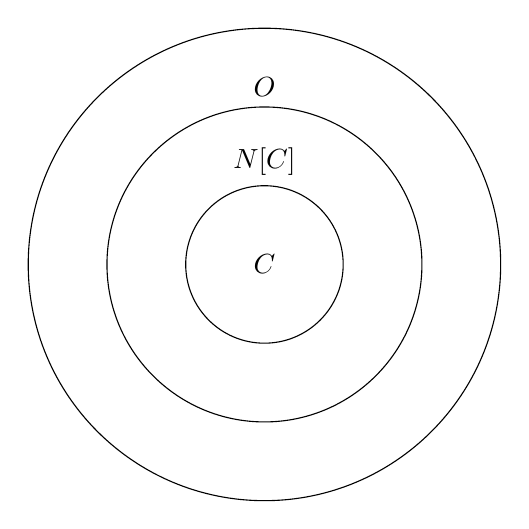
\begin{tikzpicture}
  \node[draw,circle,minimum size=2cm,label={$N[C]$}] (c) at (0, 0) { $C$ };
  \node[draw,circle,minimum size=4cm,label={$O$}] (nc) at (0, 0) {};
  \node[draw,circle,minimum size=6cm] (ext) at (0, 0) {};
\end{tikzpicture}
\caption{Divisão dos vértices de um grafo de diâmetro 2 em 3 subconjuntos}
\label{fig:blocos-d2}
\end{figure}



\begin{figure}[h]
\centering
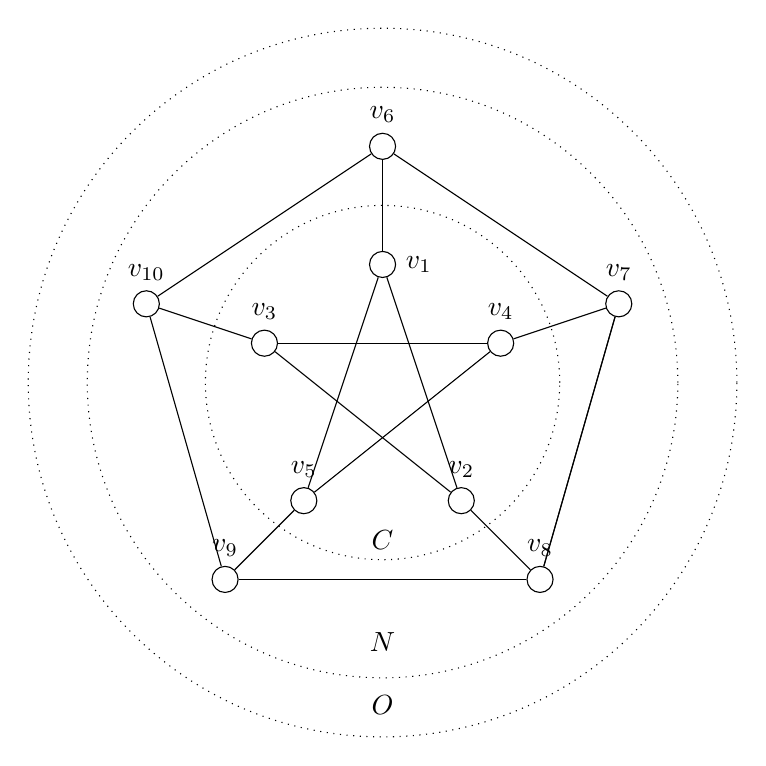
\begin{tikzpicture}
  \node[circle,draw,label=$v_6$] (v0) at (0,3.5) {};
  \node[circle,draw,label=$v_7$] (v1) at (3,1.5) {};
  \node[circle,draw,label=$v_8$] (v2) at (2,-2) {};
  \node[circle,draw,label=$v_9$] (v3) at (-2,-2) {};
  \node[circle,draw,label=$v_{10}$] (v4) at (-3,1.5) {};
  \node[circle,draw,label=right:$v_1$] (v5) at (0,2) {};
  \node[circle,draw,label=$v_4$] (v6) at (1.5,1) {};
  \node[circle,draw,label=$v_2$] (v7) at (1,-1) {};
  \node[circle,draw,label=$v_5$] (v8) at (-1,-1) {};
  \node[circle,draw,label=$v_3$] (v9) at (-1.5,1) {};

  \draw  (v0) edge node{} (v1);
  \draw  (v0) edge node{} (v4);
  \draw  (v0) edge node{} (v5);
  \draw  (v1) edge node{} (v2);
  \draw  (v1) edge node{} (v2);
  \draw  (v1) edge node{} (v6);
  \draw (v2) edge node{} (v3);
  \draw  (v2) edge node{} (v7);
  \draw  (v3) edge node{} (v4);
  \draw  (v3) edge node{} (v8);
  \draw  (v4) edge node{} (v9);
  \draw  (v5) edge node{} (v7);
  \draw  (v5) edge node{} (v8);
  \draw  (v6) edge node{} (v8);
  \draw  (v6) edge node{} (v9);
  \draw  (v7) edge node{} (v9);
  
  \node[] () at (0,-1.5) {$C$};
  \node[] () at (0,-2.8) {$N$};
  \node[] () at (0,-3.6) {$O$};
  
  \node[draw,circle,dotted,minimum size=4.5cm] (c) at (0, 0.5) {};
  \node[draw,circle,dotted,minimum size=7.5cm] (c) at (0, 0.5) {};
  \node[draw,circle,dotted,minimum size=9cm] (c) at (0, 0.5) {};
\end{tikzpicture}
\caption{Uma divisão do grafo de Petersen em conjuntos $C$, $N$ e $O$}
\label{fig:blocos-d2-petersen}
\end{figure}


Seja agora, o grafo $G_2$ da Figura~\ref{fig:blocos-d2-g2}. Dependendo de como $C$ é gerado podemos ter diferentes situações nos demais conjuntos. Por exemplo, considerando o ciclo $\{v_6v_2v_3v_4v_7\}$, podemos dividir os vértices em três subconjuntos $C=\{v_6, v_2, v_3, v_4, v_7\}$, $N=N(C) \setminus C=\{v_1, v_5\}$ e $O=\emptyset$, conforme podemos ver na Figura~\ref{fig:blocos-d2-g2}(a). Partindo de um conjunto inicial diferente, $C=\{v_1,v_2,v_6\}$, temos os subconjuntos , $N=N(C) \setminus C=\{v_3,v_5,v_7\}$ e $O=\{v_4\}$, conforme Figura \ref{fig:blocos-d2-g2}(b). Podemos observar que quando $O$ é vazio, o conjunto $C$ é um conjunto dominante.


\begin{figure}[h]
\centering
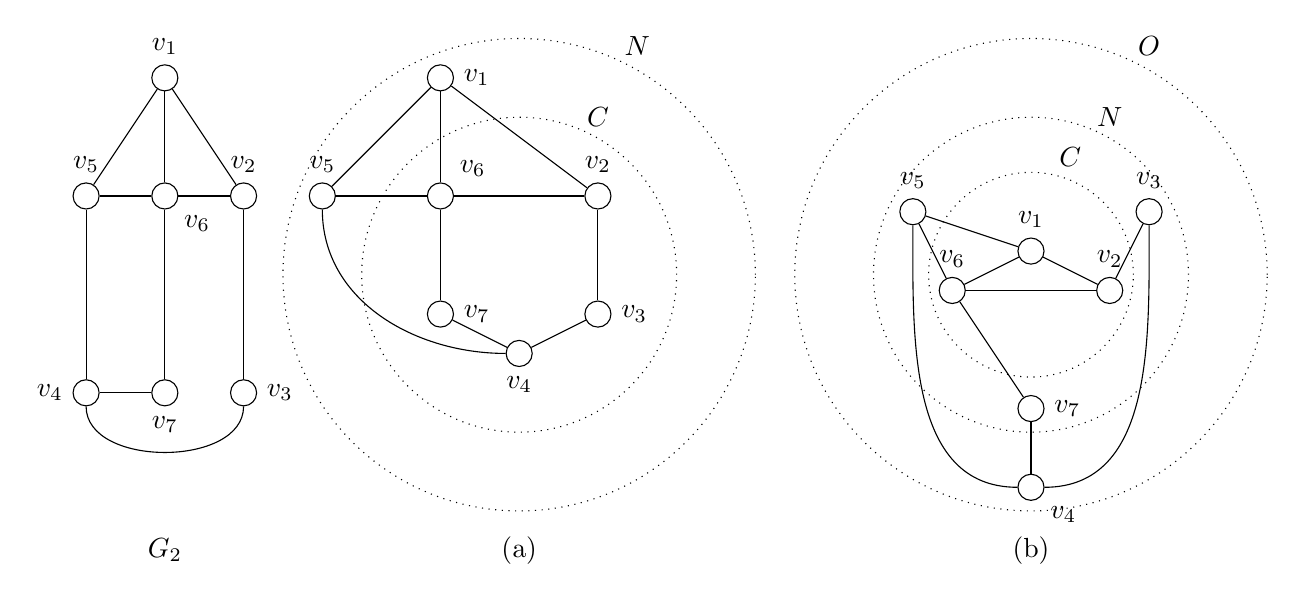
\begin{tikzpicture}
  \node[circle,draw,label=$v_1$] (v1) at (-5,2.5) {};
  \node[circle,draw,label=$v_2$] (v2) at (-4,1) {};
  \node[circle,draw,label=right:$v_3$] (v3) at (-4,-1.5) {};
  \node[circle,draw,label=left:$v_4$] (v4) at (-6,-1.5) {};
  \node[circle,draw,label=$v_5$] (v5) at (-6,1) {};
  \node[circle,draw,label=below right:$v_6$] (v6) at (-5,1) {};
  \node[circle,draw,label=below:$v_7$] (v7) at (-5,-1.5) {};

  \draw  (v1) edge (v2);
  \draw  (v2) edge (v3);		
  \draw[out=270,in=270]  (v3) edge (v4);  
  \draw  (v4) edge (v5);
  \draw  (v5) edge (v1);
  \draw  (v2) edge (v6);  
  \draw  (v4) edge (v7);  
  \draw  (v6) edge (v7);  	
  \draw  (v6) edge (v5);  
  \draw  (v6) edge (v1); 

  \node[circle,draw,label=right:$v_1$] (v11) at (-1.5,2.5) {};
  \node[circle,draw,label=$v_2$] (v12) at (0.5,1) {};
  \node[circle,draw,label=right:$v_3$] (v13) at (0.5,-0.5) {};
  \node[circle,draw,label=below:$v_4$] (v14) at (-0.5,-1) {};
  \node[circle,draw,label=$v_5$] (v15) at (-3,1) {};
  \node[circle,draw,label=above right:$v_6$] (v16) at (-1.5,1) {};
  \node[circle,draw,label=right:$v_7$] (v17) at (-1.5,-0.5) {};

  \draw  (v11) edge (v12);
  \draw  (v12) edge (v13);
  \draw  (v13) edge (v14);  
  \draw[out=180,in=270]  (v14) edge (v15);
  \draw  (v15) edge (v11);
  \draw  (v12) edge (v16);  
  \draw  (v14) edge (v17);  
  \draw  (v16) edge (v17);  
  \draw  (v16) edge (v15);  
  \draw  (v16) edge (v11); 


  \node[circle,draw,label=$v_1$] (v21) at (6,0.3) {};
  \node[circle,draw,label=$v_2$] (v22) at (7,-0.2) {};
  \node[circle,draw,label=$v_3$] (v23) at (7.5,0.8) {};
  \node[circle,draw,label=below right:$v_4$] (v24) at (6,-2.7) {};
  \node[circle,draw,label=$v_5$] (v25) at (4.5,0.8) {};
  \node[circle,draw,label=$v_6$] (v26) at (5,-0.2) {};
  \node[circle,draw,label=right:$v_7$] (v27) at (6,-1.7) {};

  \draw  (v21) edge (v22);
  \draw  (v22) edge (v23);
  \draw[out=270,in=0] (v23) edge (v24);  
  \draw[out=180,in=270]  (v24) edge (v25);
  \draw  (v25) edge (v21);
  \draw  (v22) edge (v26);  
  \draw  (v24) edge (v27);  
  \draw  (v26) edge (v27);  
  \draw  (v26) edge (v25);  
  \draw  (v26) edge (v21); 

  \draw[dotted]  (-0.5,0) ellipse (2 and 2);
  \draw[dotted]  (-0.5,0) ellipse (3 and 3);
  \draw[dotted]  (6,0) ellipse (1.3 and 1.3);
  \draw[dotted]  (6,0) ellipse (2 and 2);
  \draw[dotted]  (6,0) ellipse (3 and 3);
  
  \node at (-0.5,-3.5) {(a)};
  \node at (6,-3.5) {(b)};
  \node at (-5,-3.5) {$G_2$};

  \node at (0.5,2) {$C$};
  \node at (1,2.9) {$N$};
  
  \node at (6.5,1.5) {$C$};
  \node at (7,2) {$N$};
  \node at (7.5,2.9) {$O$};
\end{tikzpicture}
\caption{Duas possíveis divisões do grafo $G_2$ em conjuntos $C$, $N$ e $O$}
\label{fig:blocos-d2-g2}
\end{figure}


Vamos observar uma outra importante propriedade desses conjuntos, considerando a envoltória convexa. Seja $G$ um grafo de diâmetro 2, $S\subset V(G)$, e considere os subconjuntos $C=H(S)$, $N=N(C) \setminus C$ e $O= V(G) \setminus N[C]$. Caso $O$ seja vazio então a envoltório convexa de $S$ é dominante. Caso contrário, todo vértice $o \in O$ necessita ter um vizinho distinto para cada vértice em $C$, isto é $d(o)\ge |C|$. Consequentemente, se $d(o) < |C|$ então $o\not\in O$. Demonstraremos com base nas propriedades de um grafo de diâmetro 2 e no principio da casa dos pombos.

\begin{proposition}
Seja $G$ um grafo de diâmetro 2 e $S \subseteq V(G)$. Considere $C=H(S)$, $N=N(C) \setminus C$ e $O=V(G) \setminus N[C]$.
\begin{enumerate}[label=(\alph*)]
  \item{Se $O$ é vazio então $H(S)$ é dominante.} 
  \item{Se $o \in O$ então $d(o) \ge |H(S)|$.}
\end{enumerate}
\label{prop-div-conjuntos}
\end{proposition}
\begin{proof}
Como $O$ é um conjunto vazio, então pela Proposição \ref{prop:CNO} ou $v \in H(S)$ ou $v \in N$. Pela definição dos conjuntos $C$ e $N$, $H(S)$ é dominante, concluindo o item (a).

Supomos por contradição que $o\in O$ e $d(o) < |H(S)|$. Pela definição do conjunto $O$, $o$ não é adjacente a nenhum vértice em $H(S)$. Como $G$ é um grafo de diâmetro 2 todo vértice em $H(S)$ é adjacente a pelo menos um vértice em $N(o)$. Como $d(o) < |H(S)|$ temos que pelo menos um vértice $v \in N[C] \cap N[O]$ tal que $|N[v] \cap C| \geq 2$. Logo, $v \in H(S)$ e $o \in N[C]$. Uma contradição, concluindo o item (b).
%Pelo principio da casa dos pombos $\exists v \in N(o)$ tal que $d(v)=\Big\lceil\frac{|H(S)|}{d(o)}\Big\rceil$, como $|H(S)|>d(o)$ então $\frac{|H(S)|}{d(o)}>1$ e consequentemente $\Big\lceil\frac{|H(S)|}{d(o)}\Big\rceil\ge 2$, ou seja o vértice $o$ possui um vizinho $v$ que está ligado a pelo menos dois vértices em $H(S)$, esse vizinho $v$ por ter dois vértices em $H(S)$ então $v\in H(S)$, se $v\in H(S)$ então $o$ possui um vizinho em $H(S)$, consequentemente $o\in N$ e $o\not\in O$, o que é uma contradição, concluímos assim a parte (b) da proposição.
\end{proof}

%Como exemplo da Proposição~\ref{prop-div-conjuntos}(b), observemos a Figura~\ref{fig-delta-maior-hs}, temos três vértices em $H(S)$, no primeiro caso temos um vértice $o\in O$ de grau três, pelo principio da casa dos pombos cada vértice adjacente de $o$ pode ser adjacente a apenas um vértice em $H(S)$, no exemplo temos $h_1n_1,h_2n_2,h_3n_3\in E(G)$. No segundo caso temo um vértice $o\in O$ de grau dois, pelo principio da casa dos pombos um dos vértices $n_1$ ou $n_2$ precisa estar ligado a dois vértices de $H(S)$, dessa forma esse vértice estará obrigatoriamente em $H(S)$, não podendo estar em $N$ e consequentemente $o$ não pode estar em $O$.


%\begin{figure}[h]
%\centering
%\begin{tikzpicture}

%\node[circle,draw,fill,label=$h_1$] (v1) at (-5,2.5) {};
%\node[circle,draw,fill,label=$h_2$] (v3) at (-5,1.5) {};
%\node[circle,draw,fill,label=$h_3$] (v5) at (-5,0.5) {};
%\node[circle,draw,fill,fill=black!50,label=$n_1$] (v2) at (-3.5,2.5) {};
%\node[circle,draw,fill,fill=black!50,label=$n_2$] (v4) at (-3.5,1.5) {};
%\node[circle,draw,fill,fill=black!50,label=$n_3$] (v6) at (-3.5,0.5) {};
%\node[circle,draw,label=$o$] (v7) at (-2,1.5) {};

%\node[circle,draw,fill,label=$h_1$] (v9) at (0,2.5) {};
%\node[circle,draw,fill,label=$h_2$] (v13) at (0,1.5) {};
%\node[circle,draw,fill,label=$h_3$] (v10) at (0,0.5) {};
%\node[circle,draw,fill,fill=black!50,label=$n_1$] (v8) at (1.5,2.5) {};
%\node[circle,draw,fill,fill=black!50,label=$n_2$] (v11) at (1.5,0.5) {};
%\node[circle,draw,label=$o$] (v12) at (3,1.5) {};

%\draw  (v1) edge (v2);
%\draw  (v3) edge (v4);
%\draw  (v5) edge (v6);
%\draw  (v2) edge (v7);
%\draw  (v4) edge (v7);
%\draw  (v6) edge (v7);
%\draw  (v8) edge (v9);
%\draw  (v10) edge (v11);
%\draw  (v8) edge (v12);
%\draw  (v11) edge (v12);
%\draw[dotted]  (v13) edge (v11);
%\draw[dotted]  (v13) edge (v8);

%\node at (-5,3.5) {$H(S)$};
%\node at (-3.5,3.5) {$N$};
%\node at (-2,3.5) {$O$};
%\node at (0,3.5) {$H(S)$};
%\node at (1.5,3.5) {$N$};
%\node at (3,3.5) {$O$};

%\node at (-3.5,-0.5) {$d(o)\ge|H(S)|$};
%\node at (1.5,-0.5) {$d(o)<|H(S)|$};

%\draw[dotted]  (-5,1.5) ellipse (0.5 and 1.5);
%\draw[dotted]  (3,1.5) ellipse (0.5 and 1.5);
%\draw[dotted]  (1.5,1.5) ellipse (0.5 and 1.5);
%\draw[dotted]  (0,1.5) ellipse (0.5 and 1.5);
%\draw[dotted]  (-2,1.5) ellipse (0.5 and 1.5);
%\draw[dotted]  (-3.5,1.5) ellipse (0.5 and 1.5);
%\end{tikzpicture}
%\caption{Requisito necessário para vértice $o\in O$}
%\label{fig-delta-maior-hs}
%\end{figure}


Partindo da Proposição~\ref{prop-div-conjuntos}, é possível construirmos um algoritmo que iterativamente escolhe vértices em $V(G)$ para compor um conjunto $C$, tal que $C$ seja dominante. Considere um conjunto $S^\prime$ e $C=H(S^\prime)$. Podemos observar que $N=N[C] \setminus C$ é o conjunto dos vértices dominados por $H(S^\prime)$ e todo vértice $v$ do conjunto $O=N[N] \setminus N[C]$ satisfaz $d(v)\geq H(S')$. Quando a cardinalidade de $H(S^\prime)$ for maior do que $\Delta$, não existirá vértice em $O$ e consequentemente $H(S^\prime)$ é um conjunto dominante. Nesse caso, $H(S^\prime)$ será um conjunto dominante e pelo Lema~\ref{hs-dominante-envoltorio} é possível exibir um conjunto envoltório de cardinalidade $|S'|+1$. Verificaremos posteriormente que a cardinalidade máxima de qualquer $S'$ calculado pelo algoritmo será $\Big\lceil \lg{(\Delta(G) + 1)} \Big\rceil$.


O Algoritmo~\ref{alg:conjunto-envoltoria-dominante} irá de forma iterativa selecionando vértices para compor um conjunto $S^\prime$ tal que $H(S^\prime)$ é dominante. Nas linhas de 1-3 são inicializadas os conjuntos $S^\prime$, $N$ e $O$. Na Linha 4 temos o início de um laço que só finalizará quando o conjunto $O$ for vazio. Conforme vimos anteriormente se particionaremos um conjunto de vértices de um grafo seguindo as operações descritas, $O$ será vazio quando tivermos um conjunto dominante.

O Algoritmo inicia-se incluindo qualquer vértice $v \in V(G)$ em $S'$ e calcula os conjuntos $H=H(S')$, $N$ e $O$. Enquanto $O \neq \emptyset$ o algoritmo seleciona um vértice qualquer de $O$, adiciona-o em $S'$ e calcula os conjuntos $H, N$ e $O$. O processo iterativo finaliza quando $O$ for vazio e o algoritmo retorna o conjunto dominante $S'$. %Na primeira iteração do laço teremos um vértice $v$ qualquer selecionado de $O$ na linha 5, esse vértice será adicionado a $S^\prime$ na linha 6. Ainda na primeira iteração a envoltória convexa do atual conjunto $S^\prime$ será obtida na linha 7, para então nas duas linhas seguintes conseguirmos obter o conjunto $N$ dos vértices dominados e conjunto $O$ dos vértices não dominados. Ao final da primeira iteração teremos um vértice $v$ em $S^\prime$, sua vizinhança em $N=N(v)$ e em $O$ os demais vértices de $G$.


\begin{algorithm2e}[H]
    \SetAlFnt{\tiny}
    \SetAlCapFnt{\small}
    \SetAlCapNameFnt{\small}
    \SetAlgoLined
    \DontPrintSemicolon
    \LinesNumbered
    \SetAlgoLined
    \BlankLine
    \Entrada{$G(V,E)$}
    \Saida{$S^\prime$ tal que $N(H(S^\prime)) = V(G)$}
    \BlankLine
    %$i \gets 0 $\\
    $S^\prime \gets \emptyset$ \\
    $H \gets \emptyset$ \\
    $O \gets V$ \\
    \Enqto{$O \ne \emptyset$}{
         %$v \gets v\in O $\\
         %$i \gets i + 1 $\\         
         $S^\prime \gets S^\prime \cup \{ v \} | v \in O$\\
         $H \gets H(S^\prime)$ \\
         %$N \gets N(H) \setminus H$ \\
		 $O \gets V \setminus N[H]$ \\
    }
    \Retorna{$S^\prime$} 
\caption{$ConjuntoFechoDominante(G(V,E))$}
\label{alg:conjunto-envoltoria-dominante}
\end{algorithm2e} 

%Se o conjunto $O$ não é vazio, então na próxima iteração um novo vértice $v$ será selecionado, como ele não é adjacente a outros vértices em $H(S^\prime)$, $v$ precisa ao menos ter um vizinho único para cada vértice em $H(S^\prime)$. Com isso temos que $|H(S^\prime \cup \{v\})| \ge 2 \times |H(S^\prime)| + 1$. E assim sucessivamente até que $O=\emptyset$ na k-ésima iteração e por consequência $S^\prime$ é um conjunto tal que $H(S^\prime)$ é dominante. 

%\begin{lemma} 
%\end{lemma}

Para facilitar as demonstrações vamos considerar os conjuntos $S^\prime_i$, $O_i$ e $H_i$ respectivamente como os conjuntos $S^\prime$, $O$ e $H$ na i-ésima iteração do Algoritmo \ref{alg:conjunto-envoltoria-dominante}.

Considere a i-ésima iteração do Algoritmo \ref{alg:conjunto-envoltoria-dominante}. A primeira propriedade que podemos observar é que a cardinalidade do conjunto $H(S^\prime_i)$ dobra de tamanho em relação a cardinalidade do conjunto $H(S^\prime_{i-1})$.  

\begin{lemma}
Considere a i-ésima iteração do Algoritmo \ref{alg:conjunto-envoltoria-dominante}. Se $O_i \neq \emptyset$, então $|H(S^\prime_i)|\geq 2 (|H(S^\prime_{i-1})|+1)$.
\label{pior-caso-hs}
\end{lemma}
\begin{proof}
%Na primeira iteração, $S_1$ terá um vértice $v_1$, e $H(S_1)=\{v_1\}$, $N_1=N(H(S_1))=N(v_1)$ e $O_1= V\setminus N[v_1]$.
%Na segunda iteração, se $O_1 \neq \emptyset$, então um vértice $v_2 \in O_1$ será escolhido para compor o conjunto $S_2$. Observe que $v_1$ e $v_2$ não são adjacentes. Então existe pelo menos um vértice $w_1$ adjacente a ambos. Considere o conjunto $S_2=\{v_1, v_2\}$. No pior caso, $H_2=H(S_2)=\{v_1, v_2, w_1 \}$, $N_2=N(H_2)\setminus S_2$ e $O_2=V \setminus N[H_2]$.
Considere a i-ésima iteração do algoritmo. Observe que cada vértice em $O_{i}$ têm um vértice único em comum com cada vértice de $H_{i-1}$. O vértice selecionado $u \in O_{i}$ será adicionado a $S^\prime_{i}$ e todos os vértices em $N(u)\cap N(H_{i-1})$ serão incluídos em $H_{i}=H(S^\prime_i)$. Note que $|N(u)\cap N(H_{i-1})|$ será pelo menos $|H_{i-1}|$, ou seja,  $H(S^\prime_i) = H(S^\prime_{i-1}) \cup (N(u) \cap N(H_{i-1})) \cup \{u\}$. Então $|H(S^\prime_i)| = |H(S^\prime_{i-1})| + |(N(u) \cap N(H_{i-1})| + 1$. Observe que $|N(u) \cap N(H_{i-1})|$ é pelo menos $|H(S^\prime_{i-1})|$. Portanto, $|H(S^\prime_i)|\ge 2 (| H (S^\prime_ { i-1}) | +1)$.
\end{proof}

%\begin{lemma} \label{l1}
%In the worst case on a graph of diameter 2, if $O_i \neq \emptyset$, then $|H(S^\prime_i)|= 2 (|H(S^\prime_{i-1})|+1)$.
%\end{lemma}

%\begin{proof}
%At the end of the first iteration, $S_1$ will have a vertex $v_1$, $H(S_1)=\{v_1\}$, $N_1=(H(S_1))=N(v_1)$ and $O_1= V\setminus N[v_1]$.

%In the second iteration, if the set $O_1$ is not empty then a vertex $v_2 \in O_1$ will be chosen to compose the set $S_2$. Note that $v_1 $ and $v_2 $ are not adjacent. Then there exists at least one vertex $w_1$ adjacent to both. Consider the set $ S_2 = \{v_1, v_2\}$. In the worst case, $H_2=H(S_2)=\{v_1, v_2, w_1\}$, $N_2=N(H_2)\setminus S_2$ and $O_2=V\setminus N[H_2]$. 

%Observe that each vertex in $O_{i-1}$ has a unique and common vertex with each vertex of $H_{i-1}$. In the next iteration, the selected vertex $u \in O_{i-1}$ will be add to $S^\prime_{i}$ and all vertices in $N(u) \cap N(H_{i-1})$ will be included in $H_{i}=H(S^\prime_i)$. Note that $|N(u) \cap N(H_{i-1})|$ will be at least $|H(S^\prime_{i-1})|$. That is, in the worst case $H(S^\prime_i)= H(S^\prime_{i-1}) \cup (N(u) \cap N(H_{i-1})) \cup \{u\}$. So $|H(S^\prime_i)|= |H(S^\prime_{i-1})|+|(N(u) \cap N(H_{i-1})|+1$. Observe that $|(N(u) \cap N(H_{i-1})|$ is at least $|H(S^\prime_{i-1})|$. Therefore, $|H(S^\prime_i)| \ge  2 (|H(S^\prime_{i-1})|+1)$.
%\qed
%\end{proof}


Dado as garantias mínimas de crescimento de $H(S')$, provadas no Lema \ref{pior-caso-hs}, podemos analisar a progressão de crescimento da cardinalidade dos conjuntos $H$, $S$ e $O$ em cada iteração. A Tabela~\ref{tab:crescimento-envoltoria-dominante} exibe o crescimento mínimo dado pelo Lema \ref{pior-caso-hs}, dos conjuntos $H, S$ e $O$ ao longo das iterações do algoritmo. A cada iteração um novo vértice é adicionado a $S^\prime$, e $H(S^\prime)$ a cada iteração dobra a quantidade de elementos mais um. Isto é, $|H(S^\prime_i)|\ge 2 |H(S^\prime_{i-1})| +1$. %Resolvendo a relação de recorrência $T(n)\geq 2T(n-1)+1$ temos que $|H(S^\prime_i)|= T(n) \geq 2^i-1$.


 %Com a previsão minima de crescimento da cardinalidade de $H(S)$ podemos concluir que $|H(S^\prime)| > \Delta(G)$ quando $2^i-1\ge\Delta(G)$. Ou seja sabemos que $G$ possui um conjunto $S^\prime$ de cardinalidade $|S^\prime|=\Big\lceil \lg{(\Delta(G) + 1)} \Big\rceil$ tal que a envoltória de $S^\prime$ é dominante.

\begin{table}[h]
\centering
\begin{tabular}{llllll}
  \hline\noalign{\smallskip}
  \# & $S$ & $|S^\prime|$ & $H$ & $Min(|H|)$  & O  \\ 
  \noalign{\smallskip}
  \hline
  \noalign{\smallskip}
  0 & $\emptyset$ & 0 & $\emptyset$ & 0 & V(G)  \\
  1 & $\{v_1\}$   & 1 & $\{v_1\}$   & 1 & $V(G) \setminus N[H(\{v_1\})]$ \\
  2 & $\{v_1,v_2\}$ & 2 & $\{v_1,v_2,x_1\}$ & 3 & $V(G) \setminus N[H(\{v_1,v_2\})]$ \\
  3 & $\{v_1,v_2,v_3\}$ & 3 & $\{v_1,v_2,v_3,\dots,x_4\}$ & 7 & $V(G) \setminus N[H(\{v_1,v_2,v_3\})]$ \\
  \vdots & \vdots & \vdots & \vdots & \vdots & \vdots  \\
  $k$  & $\{v_1,\dots,v_k\}$ &  $k$  & $\{v_1,\dots,x_{2^k-1-k}\}$ & $2^k-1$  &  $\emptyset$ \\ \hline
\end{tabular}
\caption{Crescimento dos conjuntos $S'$, $H$ e $O$.}
\label{tab:crescimento-envoltoria-dominante}
\end{table}

Quando a cardinalidade de $H(S^\prime)$ for maior que $\Delta$, pela Proposição~\ref{prop-div-conjuntos} podemos concluir que $H(S^\prime)$ é um conjunto dominante. Logo, queremos verificar qual o máximo de iterações para que isso ocorra.

\begin{proposition} No máximo haverá $k= \Big\lceil \lg{(\Delta(G) + 1)} \Big\rceil$ iterações.
\label{max-itera}
\end{proposition}
\begin{proof}
Através do Lema~\ref{pior-caso-hs} em cada iteração do algoritmo $|H(S^\prime_i)|$ é pelo menos $2|H(S^\prime_{i-1})|+1$.
Mesmo no pior caso do Algoritmo~\ref{alg:conjunto-envoltoria-dominante} temos um crescimento exponencial de $H(S^\prime_i)$.
Resolvendo a recorrência, $T(n)\geq 2 \cdot T(n-1)+1$, a cardinalidade do conjunto pode ser dada pela equação $|H(S^\prime_i)|\geq 2^i-1$. 

Sabemos também pela Proposição~\ref{prop-div-conjuntos}, que os vértices em $O_i$ devem ter grau maior que a cardinalidade de $H(S^\prime_{i-1})$. Portanto, $O_i$ obrigatoriamente será vazio quando $H(S^\prime_{i-1})$ for maior do que $\Delta$, ou seja, quando $2^k \geq \Delta + 1$. Isolando $k$, temos que $k \geq \lg(\Delta + 1)$. Logo $k=\Big\lceil \lg{(\Delta(G) + 1)} \Big\rceil$.
\end{proof}
%existirá um conjunto $|S|=k=\left \lceil \lg {\Delta + 1)} \right\rceil$ com $H(S)$ dominante. Pelo Lema~\ref{hs-dominante-envoltorio} temos um conjunto envoltório de cardinalidade $\left \lceil \lg {\Delta + 1)} \right\rceil +1$. Com isso temos,
%\begin{equation}
%h(G) \le \left\lceil \lg{(\Delta + 1)} \right\rceil + 1
%\end{equation}
%\end{proof}

%Como em cada iteração do algoritmo o conjunto $$

\begin{coro}
Seja $G$ um grafo de diâmetro 2 biconexo então $h(G) \le \Big\lceil \lg{(\Delta(G) + 1)} \Big\rceil + 1$.
\label{coro-env-gd2}
\end{coro}
\begin{proof}
Pela Proposição \ref{max-itera}, o Algoritmo \ref{alg:conjunto-envoltoria-dominante} executa no máximo $\Big\lceil \lg{(\Delta(G) + 1)} \Big\rceil + 1$ iterações. A cada laço do algoritmo o conjunto $S'$ é incrementado de 1. Assim $|S^\prime| \leq \Big\lceil \lg{(\Delta(G) + 1)} \Big\rceil + 1$ e $H(S')$ será um conjunto dominante.  Pelo Lema~\ref{hs-dominante-envoltorio} temos um conjunto envoltório de cardinalidade $\left \lceil \lg {\Delta + 1)} \right\rceil +1$. Logo, $h(G) \le \left\lceil \lg{(\Delta + 1)} \right\rceil + 1$.

%$$ h(G) \le \Big\lceil \lg{(\Delta(G) + 1)} \Big\rceil + 1 $$

%By Lemma \ref{l1}, at each iteration $|H(S^\prime_i)|=2|H(S^\prime_{i-1})|+1$. Therefore, in the worst case, the growth of the cardinality of $ H (S) $ is exponential at each iteration, see Table \ref{table1}, and can be given by the equation $|H(S^\prime_i)|=2^i-1 $. We also note that at each iteration the set $ O_i $ is reduced proportionally, and for a vertex to be $O_i$ it must necessarily have a degree greater than the cardinality of $H(S^\prime_i)$ and have no neighbor and $H(S^\prime_i)$.

%In worst case $O_k$ will be empty when $H(S_k)$ is greater than $\Delta$. That is, when $2^k > \Delta +1$, there will be a set $S$, with $|S|=k= \left \lceil \lg {\Delta + 1)} \right\rceil$, and $H(S)$ will be a dominating set. So, by Lemma \ref{hs-dominante-envoltorio} there is a hull set of cardinality $\left \lceil \lg {\Delta + 1)} \right\rceil +1$. Therefore,

%\begin{equation}
%h(G) \le \left\lceil \lg{(\Delta + 1)} \right\rceil + 1
%\end{equation}
\end{proof}

Dessa forma temos um limite melhor para os grafos gerais de diâmetro 2 biconexos. Pelos Corolários \ref{coro-deltinha}, \ref{coro-domina1} e \ref{coro-domina2} o melhor resultado para grafo Hoffman-Singleton é um limite de 8. Em todo caso, pelo Corolário ~\ref{coro-env-gd2} esse limite é $\Big\lceil \lg{(7 + 1)} \Big\rceil + 1=4$ que confirma ser o limite superior desse parâmetro para esse grafo.

Apesar do problema de determinar se um grafo $G$ possui um conjunto entolvótorio de cardinalidade $k$, mesmo para grafos de diâmetro 2 biconexo, podemos concluir que é possível construir um conjunto envoltório em tempo polinomial de tamanho $k$, se $k \ge \left\lceil \lg{(\Delta + 1)} \right\rceil + 1$, com isso concluímos que o número envoltório para grafos de diâmetro 2 biconexo é um problema pseudo-polinomial, ou Quasi-P.

Nas próximas seções melhoraremos o limite do número envoltório para algumas subclasses de grafos de diâmetro 2.


\section{Envoltória $P_3$ para Grafos Maximais Sem Triângulo}

Os grafos maximais sem triângulo são grafos de diâmetro 2 e, conforme definido anteriormente, são minimais 2-diâmetro, isto é, a remoção de qualquer aresta aumenta o diâmetro do grafo. Como são maximais sem triângulo, a adição de qualquer aresta forma um triângulo. Alguns exemplos de grafos maximais sem triângulo, são, por exemplo, a estrela, o grafo bipartido completo, os grafos de Moore, dentre outros. Explorando algumas dessas propriedades podemos estabelecer um limite melhor do que o provado no Corolário \ref{coro-env-gd2} para o número envoltório dos grafos maximais sem triângulo.

Iniciaremos com algumas subclasses dos grafos maximais sem triângulo.


\begin{proposition}
    Seja $G$ um grafo maximal sem triângulo bipartido completo, em que cada partição tem ao menos 2 vértices, então $h(G) = 2$.
\label{prop-env-knn}
\end{proposition}
\begin{proof}
   Seja $G=(A, B, E)$ um grafo maximal sem triângulo bipartido completo tal que $|A|\geq 2$ e $|B|\geq 2$. Considere as duas partições $A$ e $B$ de $V(G)$. Sejam $v_1$ e $v_2$ vértices de uma mesma partição, digamos $A$. Por se tratar de um grafo bipartido completo, todos os demais vértices na partição $B$ são adjacentes a $v_1$ e $v_2$. Façamos $S=\{v_1,v_2\}$. Iremos mostrar que $S$ é um conjunto envoltório. Como todo vértice de $B$ é adjacente a $v_1$ e $v_2$ então $I(S)=B$. Como $|B| \geq 2$ e todo vértice de $A$ é adjacente a todos os vértices de $B$, temos que $A \subseteq I^2[S]$. Como $A\cup B=V(G)$ concluímos que $H(S)=V(G)$. Portanto, $S$ é um conjunto envoltório de $G$ e $h(G)=2$.
\end{proof}


No que diz respeito a estudos de conjuntos independentes dominantes, Barefoot et. al. em \cite{Barefoot1995} definiu uma família de grafos maximais sem triângulo $5-$partidos, que é uma generalização a partir de um $C_5$. Sejam $p$, $q$, $r$, $s$ e $t$ inteiros positivos e os conjuntos de vértices $P$, $Q$, $R$, $S$ e $T$ com cardinalidades $|P|=p, |Q|=q, |R|=r, |S|=s$ e $|T|=t$. Os grafos $C_5[p, q, r, s, t]$ possuem $p+q+r+s+t$ vértices e conjunto de vértices $V= P \cup Q \cup R \cup S \cup T$, tendo arestas somente entre todos os pares de vértices entre $P$ e $Q$, $Q$ e $R$, $R$ e $S$, $S$ e $T$ e $T$ e $P$. Podemos mostrar que o número envoltório para esta classe é no máximo $3$.

\begin{figure}[h]
\centering
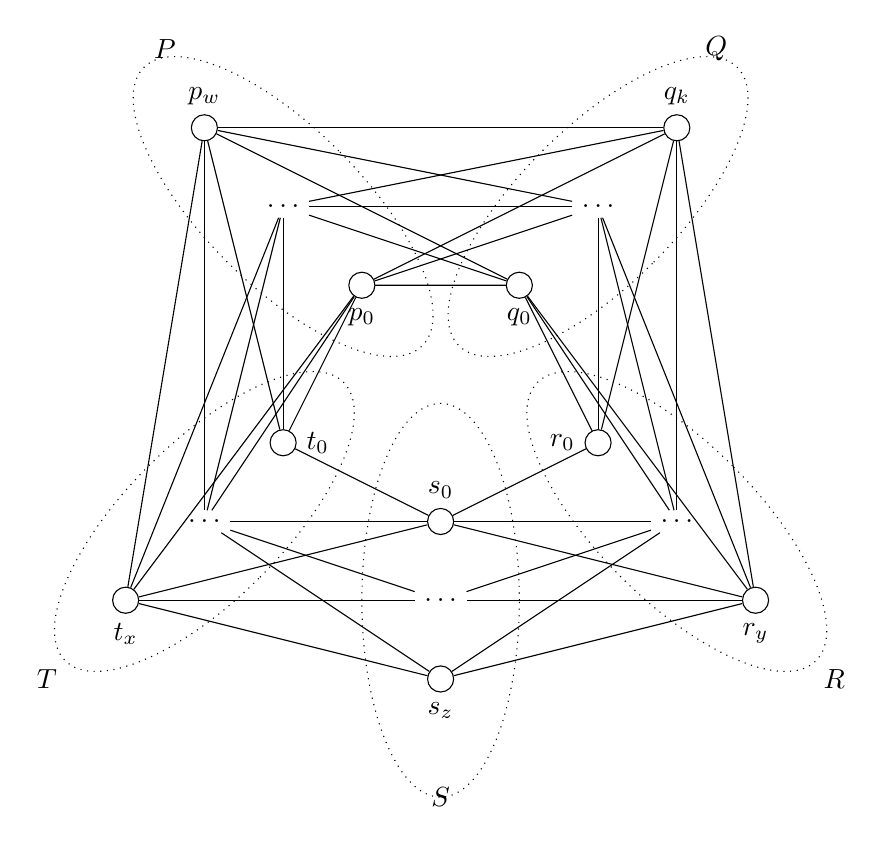
\begin{tikzpicture}
\node[draw,circle,label=$s_0$] (v4) at (-1,-4) {};
\node[circle,draw,label=right:$t_0$] (v5) at (-3,-3) {};
\node[circle,draw,label=below:$p_0$] (v1) at (-2,-1) {};
\node[circle,draw,label=below:$q_0$] (v2) at (0,-1) {};
\node[draw,circle,label=left:$r_0$] (v3) at (1,-3) {};
\draw (v1) -- (v2) -- (v3) -- (v4) -- (v5) -- (v1);
\node (v16) at (-3,0) {$\dots$};
\node[draw,circle,label=$p_w$] (v6) at (-4,1) {};
\node (v10) at (1,0) {$\dots$};
\node[draw,circle,label=$q_k$] (v9) at (2,1) {};
\node (v13) at (-1,-5) {$\dots$};
\node[draw,circle,label=below:$s_z$] (v12) at (-1,-6) {};

\node (v15) at (2,-4) {$\dots$};
\node[draw,circle,label=below:$r_y$] (v14) at (3,-5) {};
\node (v8) at (-4,-4) {$\dots$};
\node[draw,circle,label=below:$t_x$] (v7) at (-5,-5) {};

\draw  (v6) edge (v7);
\draw  (v6) edge (v8);
\draw  (v6) edge (v5);
\draw  (v6) edge (v9);
\draw  (v10) edge (v6);
\draw  (v6) edge (v2);
\draw  (v12) edge (v7);
\draw  (v13) edge (v7);
\draw  (v8) edge (v4);
\draw  (v4) edge (v7);
\draw  (v8) edge (v13);
\draw  (v8) edge (v12);
\draw  (v14) edge (v12);
\draw  (v14) edge (v13);
\draw  (v14) edge (v4);
\draw  (v15) edge (v4);
\draw  (v13) edge (v15);
\draw  (v12) edge (v15);
\draw  (v9) edge (v3);
\draw  (v9) edge (v15);
\draw  (v14) edge (v9);
\draw  (v16) edge (v9);
\draw  (v1) edge (v9);
\draw  (v10) edge (v3);
\draw  (v16) edge (v8);
\draw  (v16) edge (v7);
\draw  (v16) edge (v5);
\draw  (v16) edge (v2);
\draw  (v16) edge (v10);

\draw[dotted,rotate around={45:(-3,0)}]  (-3,0) ellipse (1 and 2.5);
\draw[dotted,rotate around={-45:(1,0)}]  (1,0) ellipse (1 and 2.5);
\draw[dotted,rotate around={-45:(-4,-4)}]  (-4,-4) ellipse (1 and 2.5);
\draw[dotted,rotate around={45:(2,-4)}]  (2,-4) ellipse (1 and 2.5);
\draw[dotted]  (-1,-5) ellipse (1 and 2.5);
\draw  (v1) edge (v7);
\draw  (v1) edge (v2);
\draw  (v14) edge (v2);
\draw  (v14) edge (v10);
\draw  (v10) edge (v15);
\draw  (v1) edge (v10);
\draw  (v1) edge (v8);
\draw  (v2) edge (v15);
\node at (-4.5,2) {$P$};
\node at (2.5,2) {$Q$};
\node at (-6,-6) {$T$};
\node at (-1,-7.5) {$S$};
\node at (4,-6) {$R$};
\end{tikzpicture}
\caption{Estrutura de um grafo MST $C_5[p, q, r, s, t]$.}
\label{fig:mst-c5}
\end{figure}


\begin{proposition}
    Se $G = C_5[p, q, r, s, t]$ então $h(G) \le 3$.
\label{coro-env-gd2-c5}
\end{proposition}
\begin{proof}
Seja $S'=\{a, b, c\}$, tal que $ab \in E(G)$ e $d(a,c)=d(b,c)=2$. Iremos exibir que $S'$ é um conjunto envoltório. Observe que $a, b$ e $c$ estão em partições diferentes. Sem perda de generalidade, considere $a \in P$, $b \in Q$ e $c \in S$. Por definição, todo vértice na partição $P$ e todo vértice na partição $S$ é adjacente a todo vértice na partição $T$. De forma análoga, todo vértice em $Q$ e todo vértice em $S$ é adjacente a todo vértice em $R$. Dessa forma, $T \cup R \subseteq I[S']$. Note que, $a$ é adjacente a todo vértice em $Q$ e todo vértice em $R$ é adjacente a todo vértice em $Q$. Então $Q \subseteq I^2[S']$. De maneira análoga, $b$ é adjacente a todo vértice em $P$ e todo vértice em $T$ é adjacente a todo vértice em $P$. Então, $P \subseteq I^2[S']$. Por fim, todo vértice em $R$ e todo vértice em $T$ é adjacente a todo vértice em $S$. Sendo assim, $S \subseteq I^2[S']$. Como $P\cup Q \cup R \cup S \cup T$ é o conjunto de vértices do grafo $C_5[p, q, r, s, t]$, concluímos que o conjunto $S'$ é um conjunto envoltório de $G$. Portanto, $h(C_5[p, q, r, s, t])\le 3$.
\end{proof}

Se a cardinalidade de cada um dos conjuntos $p, q ,r, s$ e $t$ do grafo $C_5[p,q,r,s,t]$ for maior ou igual a 2 o limite da Proposição \ref{coro-env-gd2-c5} poderá ser aperfeiçoado.

\begin{proposition}
    Se $G = C_5[p, q, r, s, t]$ e $p$, $q$, $r$, $s$ e $t$ for maior que 1 então $h(G) = 2$.
\label{coro-env-gd2-c5-h2}
\end{proposition}
\begin{proof}
Seja $S'=\{a, b\}$, tal que $a$ e $b$ estão na mesma partição. Sem perda de generalidade, considere $a,b \in P$. Por definição, todo vértice em $T$ e em $Q$ é adjacente a $a$ e $b$. Com isso $T \cup Q \subseteq I[S']$. Sejam $c$ e $d$ vértices de $Q$, todo vértice de $R$ é adjacente a $c$ e $d$, então $R \subseteq I^2[S']$. Sejam $f$ e $g$ vértices de $R$, então todo vértice de $S$ é adjacente a $f$ e $g$, com isso $S \subseteq I^2[S']$. Como $P\cup Q \cup R \cup S \cup T$ é o conjunto de vértices do grafo $C_5[p, q, r, s, t]$, concluímos que o conjunto $S'$ é um conjunto envoltório de $G$. Portanto, $h(C_5[p, q, r, s, t])= 2$.
\end{proof}

Para ilustrar, iremos utilizar o grafo $C_5[2, 2, 3, 3, 3]$ dado em \cite{Desormeaux2013,Wang2008} e representado na Figura~\ref{fig:c522333}. Considerando $S=\{p_0,q_0,s_0\}$ podemos constatar que esse conjunto é um conjunto envoltório de cardinalidade 3.% então $t_0,r_0 \in H(S)$, dessa forma temos o $C_5=p_0q_0r_0s_0t_0$ em $H(S)$, consequentemente $p_1,q_1,r1,r_2,s_1,s_2,t_1,t_2\in H(S)$. Assim sendo $H(S)=V(G)$ e $S$ é um conjunto envoltório de cardinalidade 3, conforme Teorema ~\ref{coro-env-gd2-c5}.


\begin{figure}[h]
\centering
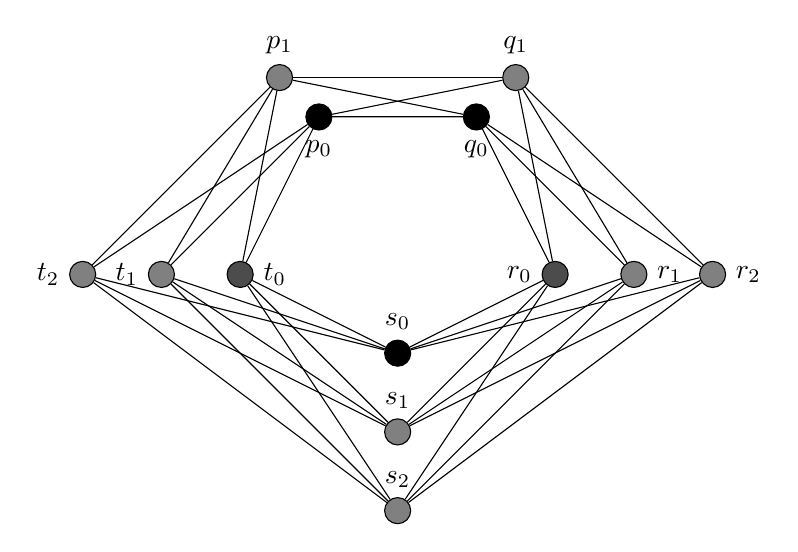
\begin{tikzpicture}
\node[draw,circle,label=$s_0$,fill] (v4) at (-1,-4) {};
\node[circle,draw,label=right:$t_0$,fill=black!70] (v5) at (-3,-3) {};
\node[circle,draw,label=below:$p_0$,fill] (v1) at (-2,-1) {};
\node[circle,draw,label=below:$q_0$,fill] (v2) at (0,-1) {};
\node[draw,circle,label=left:$r_0$,fill=black!70] (v3) at (1,-3) {};
\draw (v1) -- (v2) -- (v3) -- (v4) -- (v5) -- (v1);
\node[draw,circle,label=$p_1$,fill=black!50] (v6) at (-2.5,-0.5) {};
\node[draw,circle,label=$q_1$,fill=black!50] (v9) at (0.5,-0.5) {};
\node[draw,circle,label=$s_1$,fill=black!50] (v13) at (-1,-5) {};
\node[draw,circle,label=$s_2$,fill=black!50] (v12) at (-1,-6) {};
\node[draw,circle,label=right:$r_1$,fill=black!50] (v15) at (2,-3) {};
\node[draw,circle,label=right:$r_2$,fill=black!50] (v14) at (3,-3) {};
\node[draw,circle,label=left:$t_1$,fill=black!50] (v8) at (-4,-3) {};
\node[draw,circle,label=left:$t_2$,fill=black!50] (v7) at (-5,-3) {};
	
\draw  (v6) edge (v7);
\draw  (v6) edge (v8);
\draw  (v6) edge (v5);
\draw  (v6) edge (v9);
\draw  (v6) edge (v2);
\draw  (v12) edge (v7);
\draw  (v13) edge (v7);
\draw  (v8) edge (v4);
\draw  (v4) edge (v7);
\draw  (v8) edge (v13);
\draw  (v8) edge (v12);
\draw  (v14) edge (v12);
\draw  (v14) edge (v13);
\draw  (v14) edge (v4);
\draw  (v15) edge (v4);
\draw  (v13) edge (v15);
\draw  (v12) edge (v15);
\draw  (v9) edge (v3);
\draw  (v9) edge (v15);
\draw  (v14) edge (v9);
\draw  (v1) edge (v9);
\draw  (v1) edge (v7);
\draw  (v1) edge (v2);
\draw  (v14) edge (v2);
\draw  (v1) edge (v8);
\draw  (v2) edge (v15);
\draw  (v3) edge (v13);
\draw  (v13) edge (v5);
\draw  (v3) edge (v12);
\draw  (v12) edge (v5);
\end{tikzpicture}
\caption{Grafo $C_5[2,2,3,3,3]$ com $h(G)=2$}
\label{fig:c522333}
\end{figure}

%Triangle-free graphs and forbidden subgraphs. Stephan Brandt. Theorem 2. Let G be a triangle-free graph with at least two vertices. Then the fol- lowing four statements are equivalent: (1) every independent vertex set is contained in the neighbourhood of a vertex; (2) G is maximal triangle-free and homomorphic with ?i for some i¿1; (3) G is maximal triangle-free and does not contain an induced 6-cycle; and (4) G is maximal triangle-free and does not contain the vertex deleted Petersen graph as a (not necessarily induced) subgraph.Proof.

Em ~\cite{Brandt2002a}, temos uma ampla generalização e formas proibidas para grafos livres de triângulo. Entretanto, a mais interessante para este trabalho é a dos grafos maximais sem triângulo que não possuem um $C_6$ como subgrafo induzido. Generalizando essa propriedade para qualquer grafo de diâmetro 2, 
que não possui um $C_6$ como subgrafo induzido, podemos assim, estabelecer um melhor limite para o número envoltório.

\begin{lemma}
\label{hs-dominante-mst}     
Seja $G$ um grafo de diâmetro 2 que não possui um $C_6$ como subgrafo induzido. Então, existe $S^\prime \subseteq V(G)$ tal que $|S^\prime|=3$ e $H(S^\prime)$ é um conjunto dominante.
\end{lemma}
%\begin{proof}
%\end{proof}
%\begin{lemma}
 %    Seja $G$ um grafo de diâmetro 2 e não possui um $ciclo-6$ como subgrafo induzido então $\exists S^\prime \subseteq V(G)$ tal que $|S^\prime|=3$ e $H(S^\prime)$ é um conjunto dominante.
%\end{lemma}
\begin{proof}
Dados dois vértices de G não adjacentes $v_1$ e $v_2$, por definição $v_1$ e $v_2$ têm ao menos um vizinho em comum $x$. Com isso temos que $H(\{v_1,v_2\}$ possui ao menos três vértices, isto é, $\{v_1, v_2, x\}\subseteq H(S')$. Considere a divisão em conjuntos: $C=H(\{v_1,v_2\})$, $N=N(C)\setminus C$ e $O=N(N)\setminus N(C)$. Seja $v \in O$ e $S'=\{v_1,v_2,v\}$, vamos mostrar que $H(S')$ é um conjunto dominante.
Pela definição do conjunto $N$, todo vértice em $N$ que encontra-se dominado.

Por contradição, vamos supor que existe um vértice $u \in O$ que não é dominado por $H(S')$. Nesse caso, não existe aresta entre $u$ e $v$ e como $G$ é um grafo de diâmetro 2, existe $w\in V(G)$ tal que $w$ é adjacente a $u$ e $v$. Analisaremos individualmente as possibilidades de $w$:

{\it Caso 1:} Se $w \in N$ então necessariamente $w \in H(\{v_1,v_2,v\})$ e $u$ tem um vizinho em $H(\{v_1,v_2,v\})$, contradizendo a suposição.
    
{\it Caso 2:} Se $w \in O$, portanto, $w$ não é vizinho de $v_1$, $v_2$ ou $x$. Como $G$ é um grafo de diâmetro 2, existem os vértices $w', v'$ e $u'$ tais que $vv', v'v_1, ww', w'x, uu', u'v_2 \in E(G)$. Conforme podemos ver na Figura~\ref{fig-divisao-env-mst}. Temos com isso a formação de 2 ciclos $C_6$, o primeiro formado pelos vértices  $<v_1,v^\prime,v,w,w^\prime,x>$ e o segundo $<x,w^\prime,w,u,u^\prime,v_2>$. Considere o primeiro ciclo. Observe que $v'x,w'v_1,vw',v'w \notin E(G)$ pois, formaria um triângulo em $G$. Logo, como $G$ não possui $C_6$ como subgrafo induzido alguma aresta dentre $xv, v_1w$ e $v'w'$, deve pertencer a $E(G)$. Se $xv$ ou $w$ pertence a $E(G)$ então $v,w \in N$, o que seria uma contradição, pois, $v,w \in O$. Por exclusão, assim  $v'w'\in E(G)$. Com isso teremos $w',w\in H(\{v_1,v_2,v\})$, que implica em $u$ possuir um vizinho em $H(\{v_1,v_2,v\})$ e ser dominado, o que é uma contradição.

Por contradição em todas as possibilidades, concluímos que $H(\{v_1,v_2,v\})$ é um conjunto dominante. 
\end{proof}
   % {\it Caso 2.1:}  Se $v^\prime$ adjacente a $w^\prime$, assim $\{w^\prime,w\} \subset H(\{v_1, v_2, v \})$ implica $u$ tem vizinho $w$ em $H(\{v_1, v_2,v\})$, contradizendo a suposição.
    %Caso 2.2: Se $v^\prime$ não adjacente a $w^\prime$, então G possui um $C_6$ como subgrafo induzido, o que é uma contradição.


\begin{figure}[h]
\centering
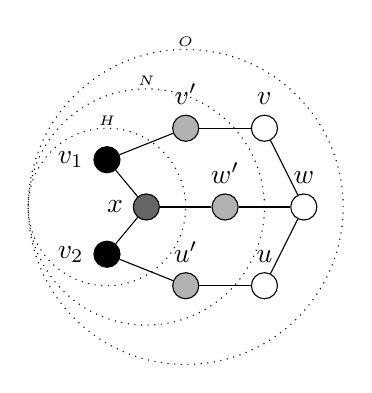
\begin{tikzpicture}
\node[circle,draw,fill=black!60,label=left:$x$] (v1) at (-1,0) {};
\node[circle,draw,fill,label=left:$v_1$] (v2) at (-1.5,0.6) {};
\node[circle,draw,fill,label=left:$v_2$] (v3) at (-1.5,-0.6) {};

\draw  (v1) edge (v2);
\draw  (v1) edge (v3);

\node[circle,draw,fill=black!30,label=$v^\prime$] (v4) at (-0.5,1) {};
\node[circle,draw,fill=black!30,label=$w^\prime$] (v9) at (0,0) {};
\node[circle,draw,fill=black!30,label=$u^\prime$] (v8) at (-0.5,-1) {};
\node[circle,draw,label=$v$] (v5) at (0.5,1) {};
\node[circle,draw,label=$w$] (v6) at (1,0) {};
\node[circle,draw,label=$u$] (v7) at (0.5,-1) {};

\draw[dotted]  (-1.5,0) ellipse (1 and 1);
\draw[dotted]  (-1,0) ellipse (1.5 and 1.5);
\draw[dotted]  (-0.5,0) ellipse (2 and 2);

\draw  (v2) edge (v4);
\draw  (v5) edge (v4);
\draw  (v5) edge (v6);
\draw  (v7) edge (v6);
\draw  (v7) edge (v8);
\draw  (v3) edge (v8);
\draw  (v6) edge (v9);
\draw  (v9) edge (v1);
\node at (-1.5,1.1) {\tiny $H$};
\node at (-1,1.6) {\tiny $N$};
\node at (-0.5,2.1) {\tiny $O$};
\end{tikzpicture}
\caption{Caso 2 do Lema~\ref{hs-dominante-mst} - Grafo sem $C_6$}
\label{fig-divisao-env-mst}
\end{figure}

\begin{coro}
    Seja $G$ um grafo de diâmetro 2 biconexo e sem $C_6$ como subgrafo. Então $h(G) \le 4$.
\label{teor-env-mst}
\end{coro}
\begin{proof}
    Pelo Lema ~\ref{hs-dominante-mst}, temos que $G$ possui um conjunto $S^\prime\subset V(G)$ tal que $|S^\prime|<=3$ e $H(S^\prime)$ é dominante. Pelo Lema ~\ref{hs-dominante-envoltorio}, temos que $\exists v \in V(G)$ tal que $S^\prime\cup\{v\}$ é envoltório. Dessa forma, temos que $G$ possui um conjunto envoltório de até quatro vértices, com isso, podemos afirmar que $h(G) \le 4$.
\end{proof}

A Figura \ref{fig-mst-h3} exemplifica um grafo $G$ com conjunto envoltório de cardinalidade 3. Como exemplo, conforme citado anteriormente, temos o grafo de Hoffman que é maximal sem triângulo, cujo número envoltória é 4. A busca por exemplos de grafos com número envoltório igual a 4 foram frustradas. O grafo de Hoffman foi o único grafo maximal sem triângulo encontrado, diferente da estrela,  cujo número envoltório é 4. Outras instâncias apresentaram grafos com número envoltório 2 ou 3. A simples obtenção de um grafo maximal sem triângulo é um trabalho árduo. Nos trabalhos de \cite{Brandt2000, BRUGMANN200951}, através de uma busca exaustiva foi possível compilar todos os grafos maximais sem triângulo de 3 até 18 vértices e estes estão disponíveis em \cite{hog2013}. Verificamos todos os grafos nessa base de dados e não encontramos exemplos cujo número envoltória fosse 4.


\begin{figure}[H]
\centering
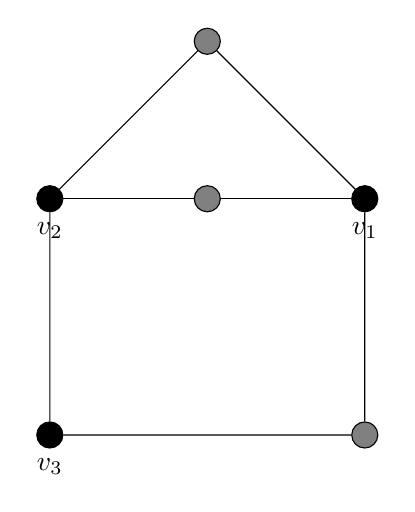
\begin{tikzpicture}
  \node[circle,draw,fill=black!50] (v9) at (0,5) {};
  \node[circle,draw,fill,label=below:$v_1$] (v10) at (2,3) {};
  \node[circle,draw,fill=black!50] (v11) at (2,0) {};
  \node[circle,draw,fill,label=below:$v_3$] (v12) at (-2,0) {};
  \node[circle,draw,fill,label=below:$v_2$] (v13) at (-2,3) {};
  \node[circle,draw,fill=black!50] (v14) at (0,3) {};
  
  \draw (v9) -- (v10) -- (v11) -- (v12) -- (v13) -- (v9);
  \draw (v13) -- (v14) -- (v10);
\end{tikzpicture}
\caption{Grafo MST com Nº Envoltório 3}
\label{fig-mst-h3}
\end{figure}

\section{Envoltória $P_3$ em Grafos Fortemente Regulares}

Um grafo $G$ é \textit{fortemente regular} se é um grafo k-regular e existem dois inteiros $b$ e $c$ tais que todos dois vértices adjacentes têm exatamente $b$ vizinhos em comum e todos dois vértices não adjacentes tenham exatamente $c$ vizinhos em comum, podendo ser definido pelos parâmetros $(n,k,b,c)$. Exemplos: Octahedral (6,4,2,4) e C5 (5,2,0,1) podem ser vistos na Figura \ref{fig:exemplos-sr} e grafos maiores como o Hoffman-Singleton (50,7,0,1), Gewirtz (56,10,0,2) e Berlekamp-van Lint-Seidel (243,22,1,2). 


\begin{figure}[h]
\centering
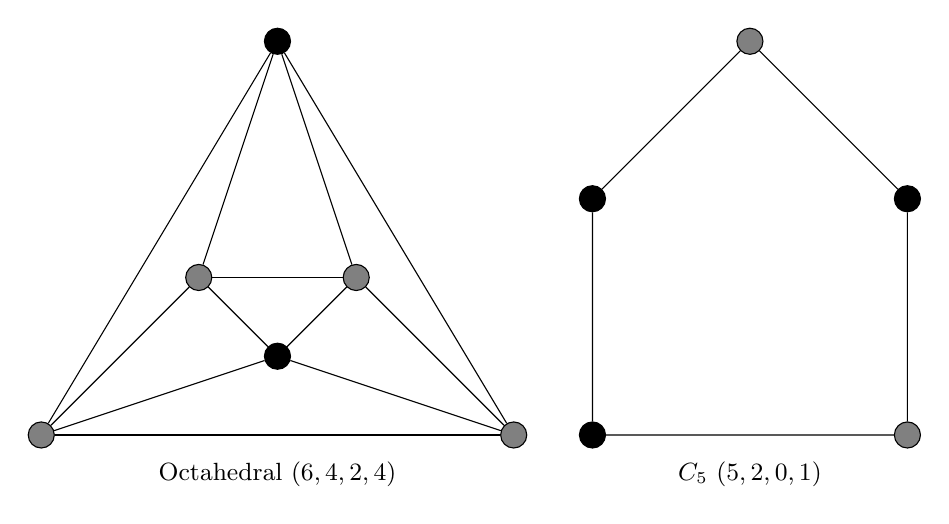
\begin{tikzpicture}
  %\node[circle,draw,fill=black!70,label=below left:$v_\delta$] (v1) at (-6,3.5) {};
  \node[circle,draw,fill] (v3) at (-6,1) {};
  \node[circle,draw,fill=black!50] (v4) at (-7,2) {};
  \node[circle,draw,fill=black!50] (v5) at (-5,2) {};
  \node[circle,draw,fill=black!50] (v6) at (-3,0) {};
  \node[circle,draw,fill=black!50] (v7) at (-9,0) {};
  \node[circle,draw,fill] (v8) at (-6,5) {};

  %\draw  (v8) edge (v1);
  %\draw  (v1) edge (v3);
  \draw  (v3) edge (v7);
  \draw  (v3) edge (v6);
  \draw  (v4) edge (v8);
  \draw  (v8) edge (v5);
  \draw  (v4) edge (v5);
  \draw  (v3) edge (v4);
  \draw  (v3) edge (v5);
  \draw  (v5) edge (v6);
  \draw  (v7) edge (v4);
  \draw  (v7) edge (v8);
  \draw  (v8) edge (v6);
  \draw  (v7) edge (v6);
  
  \node[circle,draw,fill=black!50] (v9) at (0,5) {};
  \node[circle,draw,fill] (v10) at (2,3) {};
  \node[circle,draw,fill=black!50] (v11) at (2,0) {};
  \node[circle,draw,fill] (v12) at (-2,0) {};
  \node[circle,draw,fill] (v13) at (-2,3) {};
  
  \draw (v9) -- (v10) -- (v11) -- (v12) -- (v13) -- (v9);
  
  \node at (-6,-0.5) {\small Octahedral $(6,4,2,4)$};
  \node at (0,-0.5) {\small $C_5$ $(5,2,0,1)$};
   \end{tikzpicture}
\caption{Exemplos de Grafos Fortemente Regular }
\label{fig:exemplos-sr}
\end{figure}

Inicialmente analisaremos os grafos fortemente regulares $(v,k,b,c)$, quando $c=0$. Nesse caso, o grafo é desconexo ou completo, tais como os grafos de exemplo na Figura~\ref{fig-exemplos-n-1}.

\begin{lemma}
Seja $G$ um grafo completo com $n \ge 2$ então $h(G)=2$
\label{h-kn}
\end{lemma}
\begin{proof}
Em um grafo $G$ completo quaisquer dois vértices $u$ e $v$ são adjacentes a todos os demais vértices,
ou seja, para todo $w \in V(G)\setminus \{u,v\}$ temos que $w\in N(u)\cap N(v)$ e logo $\{u,v\} \subseteq H(\{u,v\})$. Portanto, $H(\{u,v\}) = V(G)$.
\end{proof}

\begin{theorem}
\label{teor-c-0}
Seja $G$ um grafo fortemente regular $(n,k,b,c)$ com $c=0$ então $h(G)\le 2\omega(G)$.
\end{theorem}
\begin{proof}
Se $G$ é um grafo fortemente regular com $c=0$, então $G$ possui $\omega(G)$ componentes conexas. Cada componente conexa é um grafo completo com $b+1$ vértices, isto é, $K_{b+1}$. 
Um conjunto envoltório para $G$ pode ser dado pela união do conjunto envoltório de cada componente.
Como os componentes são grafos completos, sabemos pelo Lema~\ref{h-kn} que o número envoltório de cada componente é 2, portanto existe um conjunto envoltório para $G$ tal que $h(G\le 2\omega(G)$.
%Caso $\omega(G)\times 2 \ge n$ então $2\omega(G)$, como para qualquer grafo $h(G)\le n$ então vale para o caso.
%Caso $\omega(G)\times 2 < n$ então $min\{2\omega(G), n\}=2\omega(G)$, supomos por contradição que $h(G)>2\omega(G)$ então existe uma componente conexa $cc_1$ que possui $h(cc_1)\ge 3$, como $cc_1$ possui ao menos 2 vértices não adjacentes que possuem um vértice em comum, o que é uma contradição pois $c=0$.
\end{proof}



\begin{figure}[h]
\centering
\resizebox {\columnwidth} {!} {
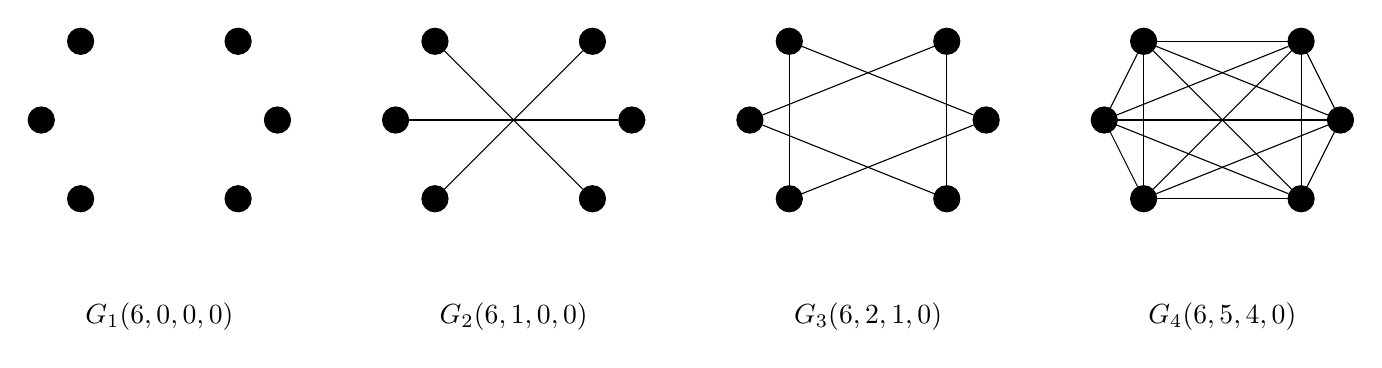
\begin{tikzpicture}
\node[circle,draw,fill] (v9) at (-19.5,-1) {};
\node[circle,draw,fill] (v5) at (-16.5,-1) {};
\node[circle,draw,fill] (v8) at (-19,-2) {};
\node[circle,draw,fill] (v6) at (-17,-2) {};
\node[circle,draw,fill] (v4) at (-17,0) {};
\node[circle,draw,fill] (v2) at (-19,0) {};
\node[circle,draw,fill] (v39) at (-15,-1) {};
\node[circle,draw,fill] (v35) at (-12,-1) {};
\node[circle,draw,fill] (v38) at (-14.5,-2) {};
\node[circle,draw,fill] (v36) at (-12.5,-2) {};
\node[circle,draw,fill] (v34) at (-12.5,0) {};
\node[circle,draw,fill] (v32) at (-14.5,0) {};
\node[circle,draw,fill] (v29) at (-10.5,-1) {};
\node[circle,draw,fill] (v25) at (-7.5,-1) {};
\node[circle,draw,fill] (v28) at (-10,-2) {};
\node[circle,draw,fill] (v26) at (-8,-2) {};
\node[circle,draw,fill] (v24) at (-8,0) {};
\node[circle,draw,fill] (v22) at (-10,0) {};
\draw  (v28) edge (v22);
\draw  (v22) edge (v25);
\draw  (v28) edge (v25);
\draw  (v29) edge (v26);
\draw  (v26) edge (v24);
\draw  (v29) edge (v24);
\draw  (v35) edge (v39);
\draw  (v36) edge (v32);
\draw  (v34) edge (v38);

\node[circle,draw,fill] (v29) at (-6,-1) {};
\node[circle,draw,fill] (v25) at (-3,-1) {};
\node[circle,draw,fill] (v28) at (-5.5,-2) {};
\node[circle,draw,fill] (v26) at (-3.5,-2) {};
\node[circle,draw,fill] (v24) at (-3.5,0) {};
\node[circle,draw,fill] (v22) at (-5.5,0) {};
\draw  (v22) edge (v24);
\draw  (v22) edge (v29);
\draw  (v22) edge (v28);
\draw  (v26) edge (v22);
\draw  (v22) edge (v25);
\draw  (v29) edge (v28);
\draw  (v28) edge (v26);
\draw  (v26) edge (v25);
\draw  (v25) edge (v24);
\draw  (v24) edge (v28);
\draw  (v24) edge (v26);
\draw  (v29) edge (v25);
\draw  (v25) edge (v28);
\draw  (v26) edge (v29);
\draw  (v24) edge (v29);

\node at (-18,-3.5) {$G_1(6,0,0,0)$};
\node at (-13.5,-3.5) {$G_2(6,1,0,0)$};
\node at (-9,-3.5) {$G_3(6,2,1,0)$};
\node at (-4.5,-3.5) {$G_4(6,5,4,0)$};
\end{tikzpicture}
}
\caption{Grafos fortemente regulares com $c=0$}
\label{fig-exemplos-c-0}
\end{figure}

Como exemplos do Teorema~\ref{teor-c-0} temos os grafos da Figura~\ref{fig-exemplos-c-0}. Para o grafo $G_1$ temos que $h(G_1) = 6 \le \omega(G_1)=12$. Considerando o grafo $G_2$ temos que $h(G_2) = 6 \leq \omega(G_2)=6$. O grafo $G_3$ apresenta $h(G_3)=4 \le \omega(G_3)=4$. Em todo caso, o grafo $G_4$ possui apenas uma componente conexa e pelo Lema~\ref{h-kn}, $h(G_4)=2$.

Os grafos fortemente regulares tal que $c>0$, são grafos conexos, não triviais, diferentes do grafo completo, grafos com diâmetro 2 e $k$-regulares. Nestes casos, o Teorema~\ref{teor-c-0} não se aplica e podemos explorar melhor essas propriedades, e estabelecer um limite melhor do que o limite para grafos de diâmetro 2 em geral. Por se tratar de um grafo de diâmetro 2, os grafos fortemente regulares conexos não tem vértices pendentes e nem vértice de corte. Com essas restrições, melhoras no limite do número envoltório podem ser estabelecidas. 

%O restante da seção será dedicada aos grafos fortemente regulares com $c> 0$, isto é, grafos conexos. Então, utilizaremos somente grafos fortemente regulares ao invés de grafos fortemente regulares conexos.

Em um grafo fortemente regular conexo a vizinhança de qualquer vértice $v$ é um conjunto dominante, pois, se $c>0$ para todo vértice $u$ não adjacente a $v$, $u$ é adjacente a $c$ vizinhos de $v$. Utilizando desta propriedade, podemos concluir que $H(N(v))$ é um conjunto dominante também.

\begin{theorem}
Seja $G$ um grafo fortemente regular $(n,k,b,c)$ com $c>0$. Então existe um $S'$ tal que $|S'| = \big\lceil \frac{k}{1+b} \big\rceil$ e $H(S')$ é um conjunto dominante.
\label{dom-gfr} 
\end{theorem}
\begin{proof}
% Para qualquer $v \in V(G)$, temos que $|N(v)|=k$. Seja $u \in N(v)$ e $S_1=\{v,u\}$. Como $u$ é adjacente a $v$ sabemos que $u$ é adjacente a $b$ dos $k$ vizinhos de $v$. Implicando que $|H(S_1)|\ge |S_1|+b=b+2$. Como $c > 0$ temos que $N(v)\not \subset |H(S_1)|$. Então, existe $w\in N(v) \setminus |H(S_1)|$ e $N(w) \cap N(u)=\{v\}$. Façamos $S_2=\{v,u,w\}$. Sabemos que $|H(S_2)| \geq |H(S_1)| + b + 1 \ge |S_2|+2b + 1$. Seguindo esse raciocínio, na $i$-ésima iteração quando $|H(S^\prime_i)|\ge k$, teremos que $N(v)\subset H(S^\prime_i)$. Logo, $|H(S^\prime_i)| \ge |S^\prime_i|+i\cdot b + 1 \ge k$. Como $|S^\prime_i|=i+1$, temos que a inequação $|H(S^\prime_i)| \ge |S^\prime_i|+i\cdot b +1 \ge k$ implica em  $i \geq \frac{k}{1+b}$. Portanto, podemos concluir que quando $i=\big\lceil \frac{k}{1+b}\big\rceil$ teremos um conjunto dominante $S^\prime_i$ tal que $S^\prime_i \leq \big\lceil \frac{k}{1+b}\big\rceil$. 
 Para qualquer $v \in V(G)$, temos que $|N(v)|=k$ e $N(v)$ é dominante. Seja $u \in N(v)$ e $S_1=\{u,v\}$. Como $u$ é adjacente a $v$ sabemos que $u$ é adjacente a $b$ dos $k$ vizinhos de $v$. Implicando que $|H(S_1)| \ge |S_1| + b$. Observe que $H(S_1)$ contém pelo menos $b+1$ vizinhos de $N(v)$. Se $N(v)\subset H(S_1)$, então $H(S_1)$ é um conjunto dominante. Caso contrário, existe $w\in N(v) \setminus H(S_1)$. Façamos $S_2=\{u,v,w\}$ então como existem $b$ vizinhos em comum entre $v$ e $w$ teremos que $|H(S_2)| \geq |H(S_1)| + (b + 1) \ge (|S_1| + b) + (b + 1)$, ou seja, $|H(S_2)| \geq 2b + 3$. 
Podemos perceber que a partir de $S_2$ o $v$ não é mais necessário, pois, $H(S_2) = H(S_2\setminus \{v\})$. Logo, vamos fazer uma redesignação de $S_2=\{u,w\}$. Com isso, $H(S_2) \geq 2b + 2$ e $H(S_2)$ contém ao menos $2b+2$ vizinhos de $v$. 
A partir de então, podemos iterar algoritmicamente, selecionando vertices $w_i \in N(v) \setminus H(S^\prime_{i-1})$ e fazendo $S^\prime_i=S^\prime_{i-1}\cup \{w_i\}$. Seguindo esse raciocínio, na $i$-ésima iteração teremos $H(S^\prime_i) \geq i \cdot b + i$. Quando $i \cdot b + i\ge k$, teremos que $N(v)\subseteq H(S^\prime_i)$. Portanto, podemos concluir que quando $i \geq \big\lceil \frac{k}{1+b}\big\rceil$ teremos um conjunto dominante $H(S^\prime_i)$ tal que $|S^\prime_i| = \big\lceil \frac{k}{1+b}\big\rceil$.

\end{proof}


\begin{coro}
Seja $G$ um grafo fortemente regular $(n,k,b,c)$ com $c>0$ então $h(G) \le \big\lceil \frac{k}{1+b} \big\rceil + 1$
\label{theor-d2-delta-sr}
\end{coro}
\begin{proof}
Seja $G$ um grafo fortemente regular $(n,k,b,c)$ com $c>0$. Pelo Teorema \ref{dom-gfr} temos que $G$ possui um conjunto dominante $S'$, tal que $|S'| = \big\lceil \frac{k}{1+b}\big\rceil$. Logo, pelo Lema \ref{hs-dominante-envoltorio}, $G$ têm um conjunto envoltório $S$ tal que $|S| \leq \big\lceil \frac{k}{1+b}\big\rceil + 1$.
%Por se tratar de um grafo fortemente regular conexo $\forall v \in V(G)$ temos que $N(v)$ é um cojunto dominante, assim se $N(v) \subset H(S^\prime)$ então $H(S^\prime)$ é dominante, como sabemos que existe um conjunto $S^\prime$ de cardinalidade $\big\lceil \frac{k}{1+b}\big\rceil$ tal que $N(v)\subset H(S^\prime)$ então pelo Lema~\ref{hs-dominante-envoltorio} temos que $G$ possui um conjunto envoltório $S$ de cardinalidade $\big\lceil \frac{k}{1+b}\big\rceil+1$,  com isso temos um limite superior para grafos fortemente regulares conexos. 
\end{proof}

Como exemplo, especificamente deste caso temos o $C_5$, que é um um grafo fortemente regular conexo. Pelo Corolário~\ref{theor-d2-delta-sr} temos que o limite superior para o seu número envoltório é $k+1=3$ e que se verifica ser o valor do seu conjunto envoltório mínimo. Na Figura~\ref{fig-exemplos-b-0-1-2} são apresentadas a vizinhanças de um vértice $v$ de três subgrafos, $G_1, G_2$ e $G_3$, que são grafos fortemente regulares, tais que $b$ é 0, 1 e 2, respectivamente. Note que $h(G_i) \leq \big\lceil \frac{k}{1+b}\big\rceil + 1$, $i=1, 2, 3$.

\begin{figure}[h]
\centering
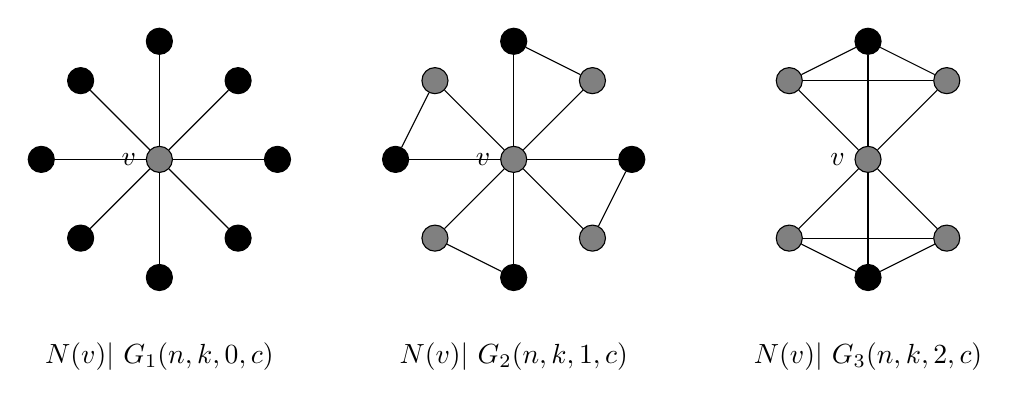
\begin{tikzpicture}
\node[circle,draw,fill=black!50,label=left:$v$] (v1) at (-13.5,-1) {};
\node[circle,draw,fill] (v3) at (-13.5,0.5) {};
\node[circle,draw,fill] (v9) at (-15,-1) {};
\node[circle,draw,fill] (v7) at (-13.5,-2.5) {};
\node[circle,draw,fill] (v5) at (-12,-1) {};
\node[circle,draw,fill] (v8) at (-14.5,-2) {};
\node[circle,draw,fill] (v6) at (-12.5,-2) {};
\node[circle,draw,fill] (v4) at (-12.5,0) {};
\node[circle,draw,fill] (v2) at (-14.5,0) {};
\draw  (v1) edge (v2);
\draw  (v1) edge (v3);
\draw  (v1) edge (v4);
\draw  (v1) edge (v5);
\draw  (v1) edge (v6);
\draw  (v7) edge (v1);
\draw  (v1) edge (v8);
\draw  (v1) edge (v9);

\node[circle,draw,fill=black!50,label=left:$v$] (v31) at (-9,-1) {};
\node[circle,draw,fill] (v33) at (-9,0.5) {};
\node[circle,draw,fill] (v39) at (-10.5,-1) {};
\node[circle,draw,fill] (v37) at (-9,-2.5) {};
\node[circle,draw,fill] (v35) at (-7.5,-1) {};
\node[circle,draw,fill=black!50] (v38) at (-10,-2) {};
\node[circle,draw,fill=black!50] (v36) at (-8,-2) {};
\node[circle,draw,fill=black!50] (v34) at (-8,0) {};
\node[circle,draw,fill=black!50] (v32) at (-10,0) {};
\draw  (v31) edge (v32);
\draw  (v31) edge (v33);
\draw  (v31) edge (v34);
\draw  (v31) edge (v35);
\draw  (v31) edge (v36);
\draw  (v37) edge (v31);
\draw  (v31) edge (v38);
\draw  (v31) edge (v39);

\node[circle,draw,fill=black!50,label=left:$v$] (v21) at (-4.5,-1) {};
\node[circle,draw,fill] (v23) at (-4.5,0.5) {};
\node[circle,draw,fill] (v27) at (-4.5,-2.5) {};
\node[circle,draw,fill=black!50] (v28) at (-5.5,-2) {};
\node[circle,draw,fill=black!50] (v26) at (-3.5,-2) {};
\node[circle,draw,fill=black!50] (v24) at (-3.5,0) {};
\node[circle,draw,fill=black!50] (v22) at (-5.5,0) {};
\draw  (v34) edge (v33);
\draw  (v36) edge (v35);
\draw  (v37) edge (v38);
\draw  (v39) edge (v32);

\node at (-13.5,-3.5) {$N(v)|$ $G_1(n,k,0,c)$};
\node at (-9,-3.5) {$N(v)|$ $G_2(n,k,1,c)$};
\node at (-4.5,-3.5) {$N(v)|$  $G_3(n,k,2,c)$};
\draw  (v22) edge (v21);
\draw  (v21) edge (v24);
\draw  (v24) edge (v22);
\draw  (v23) edge (v21);
\draw  (v22) edge (v23);
\draw  (v23) edge (v24);
\draw  (v28) edge (v21);
\draw  (v21) edge (v26);
\draw  (v27) edge (v28);
\draw  (v27) edge (v26);
\draw  (v21) edge (v27);
\draw  (v26) edge (v28);
\end{tikzpicture}
\caption{Subgrafo induzido de $N(v)$ e grafos fortemente regulares com $b=\{0,1,2\}$}
\label{fig-exemplos-b-0-1-2}
\end{figure}

O Corolário~\ref{theor-d2-delta-sr} apesar de apresentar um bom limite para certos grafos fortemente regulares não considera o parâmetro $c$. Existem grafos cuja relação dos parâmetros $k$ e $b$ não fornecem um bom limite. Como exemplo, utilizamos o grafo conhecido como $GQ(3,9)$ que possui parâmetros $(112,30,2,10)$. Segundo o limite dado pelo Corolário~\ref{theor-d2-delta-sr} temos que $h(GQ(3,9)) \leq \big\lceil \frac{k}{1+b} \big\rceil + 1=11$, porém, o valor real que computacionalmente confirmamos é $h(GQ(3,9))=2$. 

Dessa forma, vamos estabelecer um outro limite para a classe através do parâmetro $c$ e do Algoritmo \ref{alg:conjunto-envoltoria-dominante} que constrói um conjunto $S^\prime$ cujo $H(S^\prime)$ é um conjunto dominante.

%$Games$ $(729,112,1,20)$ cujo limite dado pelo Teorema~\ref{theor-d2-delta-sr} é $\big\lceil \frac{k}{1+b} \big\rceil + 1=56$ e está bem distante do valor real que computacionalmente confirmamos ser no máximo $3$. Um outro limite para a classe pode ser estabelecido partindo do parâmetro $c$ e do Algoritmo \ref{alg:conjunto-envoltoria-dominante} que constrói um conjunto $S^\prime$ cujo $H(S^\prime)$ é um conjunto dominante.


% \begin{figure}[h]
% \centering
% \begin{tikzpicture}
% \node[circle,draw] (0) at ({0*360/13}:2) {};
% \node[circle,draw] (1) at ({1*360/13}:2) {};
% \node[circle,draw] (2) at ({2*360/13}:2) {};
% \node[circle,draw] (3) at ({3*360/13}:2) {};
% \node[circle,draw] (4) at ({4*360/13}:2) {};
% \node[circle,draw] (5) at ({5*360/13}:2) {};
% \node[circle,draw] (6) at ({6*360/13}:2) {};
% \node[circle,draw] (7) at ({7*360/13}:2) {};
% \node[circle,draw] (8) at ({8*360/13}:2) {};
% \node[circle,draw] (9) at ({9*360/13}:2) {};
% \node[circle,draw] (10) at ({10*360/13}:2) {};
% \node[circle,draw] (11) at ({11*360/13}:2) {};
% \node[circle,draw] (12) at ({12*360/13}:2) {};
% \draw
% (0)--(1)--(2)--(3)--(4)--(5)--(6)--(7)--(8)--(9)--(10)--(11)--(12)--(0)
% (0)--(3)--(6)--(9)--(12)--(2)--(5)--(8)--(11)--(1)--(4)--(7)--(10)--(0)
% (0)--(4)--(8)--(12)--(3)--(7)--(11)--(2)--(6)--(10)--(1)--(5)--(9)--(0)
% ;
% \end{tikzpicture}
% \caption{Grafo 13-paley}
% \label{fig-13-paley}
% \end{figure}


Seja $G$ um grafo fortemente regular $(n,k,b,c)$ e $S' \subseteq V(G)$. Considere ainda os conjuntos $C=H(S')$, $N= N(C)\setminus C$ e $O=V(G)\setminus N[C]$. Observe que quando a cardinalidade de $H(S^\prime)$ for maior que $k$, o conjunto $O$ será vazio, caso contrário um vértice $u \in O$ teria $d(u) > k$, uma contradição, pois, $G$ é $k$-regular. Logo, pela Proposição~\ref{prop-div-conjuntos} podemos concluir que $H(S^\prime)$ é um conjunto dominante. Então, queremos verificar qual o máximo de iterações para que isso ocorra.

\begin{lemma}
Considere a i-ésima iteração do Algoritmo \ref{alg:conjunto-envoltoria-dominante} em um grafo $G$ fortemente regular $(n,k,b,c)$ com $c>0$. Se $O_i \neq \emptyset$, então $|H(S^\prime_i)|\geq (c+1) \times |H(S^\prime_{i-1})|+1$.
\label{pior-caso-hs-sr}
\end{lemma}
\begin{proof}
Considere a i-ésima iteração do algoritmo. Observe que cada vértice em $O_{i}$ têm $c$ vértices únicos, em comum com cada vértice de $H_{i-1}$. O vértice selecionado $u \in O_{i}$ será adicionado a $S^\prime_{i}$ e todos os vértices em $N(u) \cap N(H_{i-1})$ serão incluídos em $H_{i}=H(S^\prime_i)$. Note que $|N(u) \cap N(H_{i-1})|$ será $c \times |H_{i-1}|$, ou seja, $H(S^\prime_i) \supseteq H(S^\prime_{i-1}) \cup (N(u) \cap N(H_{i-1})) \cup \{u\}$. Então, $|H(S^\prime_i)| \geq |H(S^\prime_{i-1})| + |(N(u) \cap N(H_{i-1})| + |\{u\}|$. Observe que $|N(u) \cap N(H_{i-1})| = c \times |H(S^\prime_{i-1})|$. Portanto, $|H(S^\prime_i)| \ge (c+1)|H(S^\prime_{i-1})| +1$.
\end{proof}

Observe que o Lema \ref{pior-caso-hs-sr} considera somente o parâmetro $c$. Se $b=0$ na $i$-ésima iteração do Algoritmo \ref{alg:conjunto-envoltoria-dominante} teremos $|H(S^\prime_i)| = (c+1) \times |H(S^\prime_{i-1})|+1$.

\begin{proposition}
No Algoritmo~\ref{alg:conjunto-envoltoria-dominante} haverá, no máximo, $i=\big \lceil \log_{c+1}(kc+1) \big \rceil$ iterações.
\label{max-itera-sr}
\end{proposition}
\begin{proof}
Pelo Lema~\ref{pior-caso-hs-sr} em cada iteração do Algoritmo \ref{alg:conjunto-envoltoria-dominante}, $|H(S^\prime_i)|$ é pelo menos $(c+1) \times |H(S^\prime_{i-1})|+1$.
Mesmo no pior caso do Algoritmo~\ref{alg:conjunto-envoltoria-dominante} temos um crescimento exponencial de $H(S^\prime_i)$.
Resolvendo a recorrência $T(n) \geq (c+1) \cdot T(n-1) +1$, 
a cardinalidade do conjunto pode ser dada pela fórmula do somatório dos termos da progressão geométrica, obtendo a inequação $|H(S^\prime_i)| \geq \frac{(c+1)^i-1}{c} + 1$. 

Sabemos do mesmo modo pela Proposição~\ref{prop-div-conjuntos}, 
que para existir vértices em $O_i$ seu grau deve ser maior que a cardinalidade de $H(S^\prime_{i-1})$. Portanto, $O_i$ obrigatoriamente será vazio quando $H(S^\prime_{i-1})$ for maior do que $k$. Isto é, quando $\frac{(c+1)^i-1}{c} + 1 \geq k$. Isolando $i$ temos que $i \geq \log_{c+1}(kc+1)$. Logo, para $i=\Big\lceil \log_{c+1}(kc+1) \Big\rceil$ então, $H(S^\prime_i) \geq k$.
\end{proof}

Dados as garantias mínimas de crescimento de $H(S')$ provadas no Lema \ref{pior-caso-hs-sr}, podemos analisar a progressão de crescimento da cardinalidade dos conjuntos $H$, $S$ e $O$ em cada iteração. A cada iteração um novo vértice é adicionado a $S^\prime$ e a cada iteração a quantidade de elementos de $H(S^\prime)$ é multiplicada $c+1$ vezes. Isto é, $|H(S^\prime_i)| \ge (c+1) \times |H(S^\prime_{i-1})| +1$. Agora podemos utilizar o Lema \ref{hs-dominante-envoltorio} para determinar um limite para o número envoltório dos grafos fortemente regulares.

\begin{theorem}
Seja $G$ um grafo fortemente regular e $c>0$ então $h(G) \le \big \lceil \log_{c+1}(kc+1) \big \rceil + 1$.
\label{teor-d2-big-o-sr}
\end{theorem}
\begin{proof}
Pelo Lema~\ref{pior-caso-hs-sr} sabemos que $G$ possui um conjunto $S^\prime$ tal que $H(S^\prime)$ é dominante, e $|S^\prime|=\big \lceil \log_{c+1}(kc+1) \big \rceil$. Logo, pelo Lema~\ref{hs-dominante-envoltorio} temos que $h(G)\le \big \lceil \log_{c+1}(kc+1) \big \rceil + 1$.
\end{proof}

%Com o Teorema~\ref{teor-d2-big-o-sr} temos um valor alternativo para o número envoltório para grafos fortemente regular, podemos ver que para o grafo $Games$ o limite é $2$ que é melhor do que o apresentado pelo Teorema~\ref{theor-d2-delta-sr}.

Com o Teorema~\ref{teor-d2-big-o-sr} temos um valor alternativo para o limite do número envoltório para grafos fortemente regular considerando o parâmetro $c$. Podemos ver que para o grafo $GQ(3,9)$ o limite é $4$, melhor que o apresentado pelo Corolário~\ref{theor-d2-delta-sr}.

Na Tabela~\ref{tab-resultados-execucao} temos resultados comparativos para alguns grafos verificados pelo Algoritmo~\ref{alg:numero-envoltoria-p3} e os resultados teóricos encontrados neste trabalho. Na tabela, a coluna $h$ exibe o resultado obtido computacionalmente pelo Algoritmo \ref{alg:numero-envoltoria-p3}. A segunda e terceira colunas apresentam os limites apresentados, respectivamente, pelo Corolário \ref{coro-deltinha} e Corolário \ref{coro-env-gd2}. E a quarta e quinta colunas apresentam os resultados obtidos, respectivamente, pelos Corolário \ref{theor-d2-delta-sr} e Corolário \ref{teor-d2-big-o-sr}. Foram verificados aproximadamente 43.669 grafos fortemente regular conexos disponíveis em \cite{hog2013,spence12,weisstein2018}.

\begin{table}[H]
\caption{Resultados comparativos para o número envoltório}
\label{tab-resultados-execucao}
\begin{tabular}{r|c|c|c|c|c}
                            &                     & \multicolumn{2}{c|}{\textbf{Diâmetro 2}}                                                & \multicolumn{2}{c}{\textbf{Fortemente Regular}} \\ 
\textbf{Grafo}              & \textbf{h}          & \textbf{Corol.}~\ref{coro-deltinha}          & \textbf{Corol.}~\ref{coro-env-gd2}         & \textbf{Corol.}~\ref{theor-d2-delta-sr}             & \textbf{Teor.}~\ref{teor-d2-big-o-sr}  \\ \hline
$C_5$ (5,2,0,1) & 3  & 3 & 3 & 3 & 3 \\
Petersen (10,3,0,1) & 3  & 4 & 3 & 4 & 3\\
Clebsch (16,5,0,2)  & 3 & 6 & 4 & 6 & 3 \\
(4,4)-Hook (16,6,2,2) & 2  & 7 & 4 & 3 & 3\\
Hoffman-Singleton (50,7,0,1) & 4 & 8 & 4 & 8 & 4 \\
Gewirtz (56,10,0,2) & 3  & 11 & 4 & 11 & 4\\
Brouwer-Haemers (81,20,1,6) & 2 & 21 & 5 & 11 & 3\\
$M_{22}$ (77,16,0,4) & 2  & 17 & 5 & 17 & 4\\
$H(2,10)$ (100,18,8,2) & 2 & 19 & 5 & 3 & 4\\
Higman-Sims (100,22,0,6) & 2  & 23 & 6 & 23 & 4\\
$1^{st}$ sub. of McLaughlin (112,30,2,10) & 2 & 113 & 8 & 5 & 3\\
Cameron (231,30,9,3) & 2  & 31 & 6 & 4 & 4 \\
Berlekamp-van L. (243,22,1,2) & 3 & 23 & 6 & 12 & 4 \\
McLaughlin (275,112,30,56)  & 2   & 113 & 8 & 5 & 3\\
Grassmann $J_2(6,2)$ (651,90,33,9) & 2 & 91 & 8 & 4 & 4 \\	
G2(4) (416,100,36,20) & 2 & 101 & 8 & 4  & 3  \\
Games (729,112,1,20) & * &  113 & 8 & 57 & 4 \\
\end{tabular}
\end{table}

Podemos observar na Tabela \ref{tab-resultados-execucao} que o limite apresentado pelo Corolário \ref{coro-env-gd2} para grafos de diâmetro 2 é um bom limite e que atinge a igualdade para algumas classes de grafos. O limite apresentado pelo Corolário \ref{teor-d2-big-o-sr} para grafos fortemente regulares e considerando o parâmetro $c$ é melhor do que o limite considerando o parâmetro $b$.

No próximo capítulo trabalharemos com o número de Carathéodory na convexidade $P_3$ para alguns grafos de diâmetro 2.

